\section*{第八章 概率与统计}

1. C

2. $C$

3. C

4. A 提示: 若 $A,B$ 互斥,则 $P\left( {A \cap  B}\right)  = 0$ ,故 $A$ 错误.

若 $A,B$ 互斥,则 $A \subseteq  \bar{B}$ ,则 $P\left( {A \cup  \bar{B}}\right)  = P\left( \bar{B}\right)  = 1 - P\left( B\right)  = \dfrac{1}{2}$ ,故 $B$ 正确.

若 $A,B$ 独立,则 $P\left( {A \cap  \bar{B}}\right)  = P\left( A\right) P\left( \bar{B}\right)  = P\left( A\right) \left\lbrack  {1 - P\left( B\right) }\right\rbrack   = \dfrac{1}{6}$ ,故 $C$ 正确.

若 $A,B$ 独立,则 $P\left( {A \cup  B}\right)  = P\left( A\right)  + P\left( B\right)  - P\left( {A \cap  B}\right)  = \dfrac{1}{3} + \dfrac{1}{2} - \dfrac{1}{6} = \dfrac{2}{3}$ ,故 $D$ 正确.

5. D 提示: 由已知可得 $P\left( A\right)  = \dfrac{3}{6} = \dfrac{1}{2},P\left( B\right)  = \dfrac{2}{6} = \dfrac{1}{3},P\left( C\right)  = \dfrac{1}{6},P\left( {A \cap  B}\right)  = 0$ ,

$P\left( {A \cup  B}\right)  = P\left( A\right)  + P\left( B\right)  - P\left( {A \cap  B}\right)  = \dfrac{5}{6}$ , A 选项错误.

因为 $P\left( {A \cap  B \cap  C}\right)  = 0$ ,所以事件 $A,B,C$ 不可能同时发生, $B$ 选项错误.

事件 $\bar{A}$ 表示“取到的不是红球”即“取到的是黄球或白球”,事件 $\bar{B}$ 表示“取到的不是白球”即“取到的是黄球或红球”,事件 $\bar{A},\bar{B}$ 可以同时发生,即 “取到的是黄球”,不是互斥, C 选项错误.

$P\left( {A \cap  B}\right)  = 0,P\left( A\right)  = \dfrac{1}{2},P\left( B\right)  = \dfrac{1}{3},P\left( {A \cap  B}\right)$ 不等于 $P\left( A\right) P\left( B\right)$ ,事件 $A$ 与事件 $B$ 不相互独立, $D$ 选项正确.

6. D 提示: 设第一次、第二次摸球的编号分别为 $x,y$ ,则共有 12 个样本点.

事件 $A$ 包含的样本点有: $\left( {1,2}\right) ,\left( {1,3}\right) ,\left( {1,4}\right) ,\left( {2,1}\right) ,\left( {2,3}\right) ,\left( {2,4}\right)$ ,共 6 个.

事件 $B$ 包含的样本点有: $\left( {1,2}\right) ,\left( {2,1}\right) ,\left( {3,1}\right) ,\left( {3,2}\right) ,\left( {4,1}\right) ,\left( {4,2}\right)$ ,共 6 个.

事件 $A \cap  B$ 包含的样本点有: $\left( {1,2}\right) ,\left( {2,1}\right)$ ,共 2 个.

事件 $C$ 包含的样本点有: $\left( {1,2}\right) ,\left( {1,3}\right) ,\left( {1,4}\right) ,\left( {3,1}\right) ,\left( {3,2}\right) ,\left( {3,4}\right)$ ,共 6 个.

事件 $A \cap  C$ 包含的样本点有: $\left( {1,2}\right) ,\left( {1,3}\right) ,\left( {1,4}\right)$ ,共 3 个.

则 $A \cap  B \neq  \varnothing ,A \cap  C \neq  \varnothing$ ,则 $A,C$ 错误.

$P\left( A\right)  = P\left( B\right)  = \dfrac{1}{2},P\left( {A \cap  B}\right)  = \dfrac{2}{12} \neq  P\left( A\right) P\left( B\right)$ , B 错误.

$P\left( A\right)  = P\left( C\right)  = \dfrac{1}{2},P\left( {A \cap  C}\right)  = \dfrac{1}{4} = P\left( A\right) P\left( C\right) ,D$ 正确.

7. A 提示: 设该电路正常工作为事件 $D$ ,则 $P\left( D\right)  = P\left( A\right) \{ 1 - \left\lbrack  {1 - P\left( B\right) }\right\rbrack   \cdot  \left\lbrack  {1 - P\left( C\right) }\right\rbrack  \}  = \dfrac{1}{3} \times  \left\lbrack  {1 - \left( {1 - \dfrac{3}{5}}\right) \left( {1 - \dfrac{1}{2}}\right) }\right\rbrack   = \dfrac{4}{15}$ .

8. $B$ 提示: $P\left( A\right)  = 1 - \dfrac{3}{5} = \dfrac{2}{5}$ ,从而 $P\left( A\right) P\left( B\right)  = \dfrac{2}{5} \times  \dfrac{1}{4} = \dfrac{1}{10} = P\left( {A \cap  B}\right)  \neq  0$ ,故 $A$ 错误, $B$ 正确.

$P\left( {A \cup  B}\right)  = P\left( A\right)  + P\left( B\right)  - P\left( {A \cap  B}\right)  = \dfrac{2}{5} + \dfrac{1}{4} - \dfrac{1}{10} = \dfrac{11}{20}$ ,故 C 错误.

$P\left( {\bar{A} \cap  B}\right)  = P\left( B\right)  - P\left( {A \cap  B}\right)  = \dfrac{1}{4} - \dfrac{1}{10} = \dfrac{3}{20}$ ,故 D 错误.

9. C 提示: 选项 A,假设甲组的失分情况为 3, 3, 3, 3, 3, 3, 3, 3, 3, 3, 3, 满足中位数为 3, 极差为 5, 但该组不是 “优秀小组”,故 A 错误.

选项 B,假设乙组的失分情况为0,0,1,1,2,2,2,2,8,满足平均数为 2,众数为 2,但该组不是 “优秀小组”, B 错误.

选项 C,丙组的失分情况从小到大排列依次为 ${x}_{1},{x}_{2},\cdots ,{x}_{10}$ ,丙组平均数为 2,方差为 3,即 ${\left( {x}_{1} - 2\right) }^{2} + {\left( {x}_{2} - 2\right) }^{2} + \cdots  +$  ${\left( {x}_{10} - 2\right) }^{2} = {30}$ ,若 ${x}_{k} \geq  8\left( {k = 1,2,3,\cdots ,{10}}\right)$ ,则 ${\left( {x}_{k} - 2\right) }^{2} \geq  {36} > {30}$ ,不合要求,故 ${x}_{k} \leq  7$ ,

所以该组每位选手失分都不超过 7 分,则该组为 “优秀小组”,故 $C$ 正确.

选项 D,85\%×10=8.5,故从小到大,选取第 9 个数作为第 85 百分位数,即从小到大第 9 个数为 7 ,假设丁组失分情况为 0,0,0,0,0,0,0,5,7,8,满足平均数为 2,第 85 百分位数为 7,但不是“优秀小组”,故 $D$ 错误.

10. $C$ 提示: $\dfrac{1}{9}\mathop{\sum }\limits_{{i = 1}}^{9}{x}_{i} = 9,\dfrac{1}{9}\mathop{\sum }\limits_{{i = 1}}^{9}{\left( {x}_{i} - 9\right) }^{2} = \dfrac{1}{9}\left( {\mathop{\sum }\limits_{{i = 1}}^{9}{x}_{i}^{2} - 9 \times  {9}^{2}}\right)  = {12}$ ,可得 $\mathop{\sum }\limits_{{i = 1}}^{9}{x}_{i} = {81},\mathop{\sum }\limits_{{i = 1}}^{9}{x}_{i}^{2} = {837}$ ,

又 $\dfrac{1}{10}\left( {\mathop{\sum }\limits_{{i = 1}}^{9}{x}_{i} + {x}_{10}}\right)  = \dfrac{1}{10}\left( {{81} + {x}_{10}}\right)  = {10}$ ,于是 ${x}_{10} = {19}$ .

所以新样本数据的方差为 $\dfrac{1}{10}\mathop{\sum }\limits_{{i = 1}}^{{10}}{\left( {x}_{i} - {10}\right) }^{2} = \dfrac{1}{10}\left( {\mathop{\sum }\limits_{{i = 1}}^{{10}}{x}_{i}^{2} - {10} \times  {10}^{2}}\right)  = \dfrac{1}{10}\left( {\mathop{\sum }\limits_{{i = 1}}^{9}{x}_{i}^{2} + {x}_{10}^{2} - {10} \times  {10}^{2}}\right)  = {19.8}$ .

11. D 提示: 新的一组数据的平均数为 $\dfrac{2 \times  5 + 4 \times  5}{10} = 3$ ,方差为 ${s}^{2} = \dfrac{1}{2} \times  \left\lbrack  {2 + {\left( 4 - 3\right) }^{2}}\right\rbrack   + \dfrac{1}{2} \times  \left\lbrack  {4 + {\left( 2 - 3\right) }^{2}}\right\rbrack   = 4$ .

12. $C$ 提示: 该校高三年级全体学生的年龄方差为 ${s}^{2} = \dfrac{{N}_{1}}{{N}_{1} + {N}_{2}}\left\lbrack  {{s}_{1}^{2} + {\left( {\bar{x}}_{1} - \bar{x}\right) }^{2}}\right\rbrack   + \dfrac{{N}_{2}}{{N}_{1} + {N}_{2}}\left\lbrack  {{s}_{2}^{2} + {\left( \overline{{x}_{2}} - \bar{x}\right) }^{2}}\right\rbrack$ ,

当 $\overline{{x}_{1}} = \overline{{x}_{2}}$ 时, $\overline{x} = \overline{{x}_{1}} = \overline{{x}_{2}},{s}^{2} = \dfrac{{N}_{1}}{{N}_{1} + {N}_{2}}{s}_{1}^{2} + \dfrac{{N}_{2}}{{N}_{1} + {N}_{2}}{s}_{2}^{2}$ .

13. $C$ 提示: 不妨设这 5 次的分数从小到大分别为 $a,a + d,a + {2d},a + {3d},a + {4d}\left( {a > 0,d > 0}\right)$ ,所以 $\bar{x} = a + {2d}$ ,第 60 百分位数为 $m = \dfrac{a + {2d} + a + {3d}}{2} = a + \dfrac{5}{2}d$ .

要使 4 次成绩的平均分数为 $\bar{y}$ 且 $\bar{y} = \bar{x}$ ,则去掉的数据一定是 $a + {2d}$ ,即还剩下 $a,a + d,a + {3d},a + {4d}\left( {a > 0,d > 0}\right)$ . 又 $4 \times  {60}\%  = {2.4}$ ,所以第 60 百分位数为 $n = a + {3d}$ . 因为 $d > 0$ ,所以 $n > m$ .

14. C 提示: 由于 $a = 2,b = 7$ ,故从 $\{ 0,1,2\} ,\{ 3,4,5,6\} ,\{ 7,8,9\}$ 中各取一个数.

因为所组成的三位数能被 3 整除,所以所取的三个数字构成的集合可以为 $\{ 0,3,9\} ,\{ 0,4,8\} ,\{ 0,5,7\} ,\{ 0,6,9\} ,\{ 1,3,8\}$ , $\{ 1,4,7\} ,\{ 1,5,9\} ,\{ 1,6,8\} ,\{ 2,3,7\} ,\{ 2,4,9\} ,\{ 2,5,8\} ,\{ 2,6,7\}$ ,其中含 0 的每组可组成 4 个不同的三位数,不含 0 的每组可组成 6 个不同的三位数,所以共有 $4 \times  4 + 8 \times  6 = {64}$ (个)不同的三位数.

15. 79 提示:由题意得,数据的极差为 40,因为数据中最小值为 41,故 $m$ 为 ${81},{81}\%  \times  {11} = {8.91}$ ,将数据从小到大排列,可得 41,45,53,56,65,69,70,72,79,80,81,故这组数据的第 $m$ 百分位数为第九个数据 79 .

16. $\dfrac{14}{9}$ 提示:因为平均数为 $\dfrac{1 + 3 + 4 + x + y + y + 2}{6}$ ,第 50 百分位数为 $\dfrac{4 + x}{2}$ ,

所以 $y = x + 1$ ,故数据 $x,y,y + 2$ 的方差为 $\dfrac{1}{3}\left\lbrack  {{\left( x - x - \dfrac{4}{3}\right) }^{2} + {\left( x + 1 - x - \dfrac{4}{3}\right) }^{2} + {\left( x + 3 - x - \dfrac{4}{3}\right) }^{2}}\right\rbrack   = \dfrac{14}{9}$ .

17. 275 提示: 记男生样本的均值为 $\bar{y}$ ,方差为 ${s}_{1}^{2}$ ,女生样本的均值为 $\bar{z}$ ,方差为 ${s}_{2}^{2}$ ,容量为 50 的样本均值为 $\bar{x}$ ,方差为 ${s}^{2}$ ,则 $\bar{y} = {176},{s}_{1}^{2} = {100},\bar{z} = {166},{s}_{2}^{2} = {400}$ ,所以 $\bar{x} = \dfrac{25}{50} \times  {176} + \dfrac{25}{50} \times  {166} = {171}$ ,

${s}^{2} = \dfrac{25}{50}\left\lbrack  {{s}_{1}^{2} + {\left( \bar{y} - \bar{x}\right) }^{2}}\right\rbrack   + \dfrac{25}{50}\left\lbrack  {{s}_{2}^{2} + {\left( \bar{z} - \bar{x}\right) }^{2}}\right\rbrack   = \dfrac{1}{2} \times  \left( {{100} + {25}}\right)  + \dfrac{1}{2} \times  \left( {{400} + {25}}\right)  = {275}.$

18. (1) 若一次抽取 3 张卡片,样本空间为 $\{ \left( {1,2,3}\right) ,\left( {1,2,4}\right) ,\left( {1,3,4}\right) ,\left( {2,3,4}\right) \}$ .

其中事件 $A = \{ \left( {1,3,4}\right) ,\left( {2,3,4}\right) \}$ 包含 2 个样本点,所以 $P\left( A\right)  = \dfrac{2}{4} = \dfrac{1}{2}$ .

(2)若第一次抽取 1 张卡片,放回后再抽取 1 张卡片,样本空间为 $\{ \left( {m,n}\right)  \mid  m = 1,2,3,4,n = 1,2,3,4\}$ ,共包含 $4 \times  4 = {16}$ 个样本点,

其中事件 $B = \{ \left( {3,4}\right) ,\left( {4,4}\right) ,\left( {4,3}\right) \}$ 包含 3 个样本点,所以 $P\left( B\right)  = \dfrac{3}{16}$ .

(3)一次抽取 2 张卡片,样本空间为 $\{ \left( {1,2}\right) ,\left( {1,3}\right) ,\left( {1,4}\right) ,\left( {2,3}\right) ,\left( {2,4}\right) ,\left( {3,4}\right) \}$ ,共包含 6 个样本点,事件 $C =$  $\{ \left( {1,2}\right) ,\left( {2,4}\right) \}$ ,所以 $P\left( C\right)  = \dfrac{2}{6} = \dfrac{1}{3}$ ,事件 $D = \{ \left( {1,4}\right) ,\left( {2,4}\right) ,\left( {3,4}\right) \}$ ,所以 $P\left( D\right)  = \dfrac{3}{6} = \dfrac{1}{2}$ .

当 $C,D$ 同时发生时,即 2 张卡片上数字之和是 3 的倍数同时积是 4 的倍数,只有一种取法(2,4),所以 $P\left( {C \cap  D}\right)  =$  $\dfrac{1}{6}$ . 因为 $P\left( {C \cap  D}\right)  = P\left( C\right) P\left( D\right)$ ,所以事件 $C$ 与事件 $D$ 是独立的.

19. 这种说法是有道理的. 对每一名学生的视力进行调查, 这样会浪费大量的人力、物力, 如果设计合适的抽样方法, 也会得到差不多的结果, 例如, 可根据小学生、中学生、大学生进行分层抽样, 再在每一层中根据城市、农村进行抽样, 这样就具. 有代表性, 因而得到的结果比较准确.

20. (1) 因为小矩形的面积之和为 1,所以 $\left( {{0.005} + {0.010} + {0.020} + a + {0.025} + {0.010}}\right)  \times  {10} = 1$ ,则 $a = {0.030}$ .

(2)成绩落在 $\lbrack {40},{80})$ 内的频率为 $\left( {{0.005} + {0.010} + {0.020} + {0.030}}\right)  \times  {10} = {0.65}$ ,

落在 $\lbrack {40},{90})$ 内的频率为 $\left( {{0.005} + {0.010} + {0.020} + {0.030} + {0.025}}\right)  \times  {10} = {0.9}$ .

设第 75 百分位数为 $m$ ,由 ${0.65} + \left( {m - {80}}\right)  \times  {0.025} = {0.75}$ ,得 $m = {84}$ ,故第 75 百分位数的估计值为 84 .

(3) 由图可知,成绩在 $\lbrack {50},{60})$ 的市民人数为 ${100} \times  {0.1} = {10}$ ,

成绩在 $\lbrack {60},{70})$ 的市民人数为 ${100} \times  {0.2} = {20}$ ,

故这两组成绩的总平均数为 $\dfrac{{10} \times  {57} + {69} \times  {20}}{{10} + {20}} = {65}$ ,总方差为 ${s}^{2} = \dfrac{10}{30} \times  \left\lbrack  {7 + {\left( {57} - {65}\right) }^{2}}\right\rbrack   + \dfrac{20}{30} \times$

$\left\lbrack  {4 + {\left( {69} - {65}\right) }^{2}}\right\rbrack   = {37}.$

21. (1) 根据分层抽样知:应抽取小吃类 ${80} \times  \left( {1 - {30}\%  - {15}\%  - {10}\%  - 5\%  - 5\% }\right)  = {28}$ 家,

生鲜类 ${80} \times  {15}\%  = {12}$ 家,所以应抽取小吃类 28 家,生鲜类 12 家.

(2)① 根据题意可得 $\left( {{0.002} \times  3 + {2a} + {0.006}}\right)  \times  {50} = 1$ ,解得 $a = {0.004}$ .

设第 75 百分位数为 $x$ ,因为 $\left( {{0.002} + {0.004} + {0.006}}\right)  \times  {50} = {0.6}$ ,所以 $\left( {x - {450}}\right)  \times  {0.004} + {0.6} = {0.75}$ ,解得 $x =$ 487.5, 所以该直播平台商家平均日利润的第 75 百分位数为 487.5 元.

② $\left( {\dfrac{{500} - {480}}{50} \times  {0.004} + {0.002} + {0.002}}\right)  \times  {50} \times  {1000} = {280}$ ,所以估计该直播平台“优质商家”的个数为 280.

22. (1) 由题意可知,周劳动时间在 $\lbrack 3,4)$ 小时的频率为 $\dfrac{140}{500} = {0.28}$ , 周劳动时间在 $\left\lbrack  {5,6}\right\rbrack$ 小时的频率为 $\dfrac{60}{500} = {0.12}$ ,所以补全的频率分布直方图如图所示.

\begin{center}
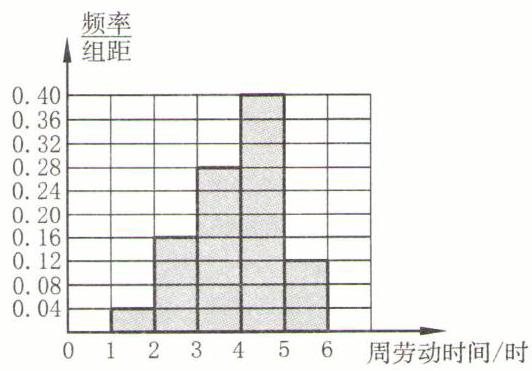
\includegraphics[width=0.4\textwidth]{bodyxb/src/bo_d20cdrf7aajc73bfmvhg_193_893_430_532_371_0.jpg}
\end{center}


(第 22 题)

(2)周劳动时间平均数为: ${1.5} \times  {0.04} + {2.5} \times  {0.16} + {3.5} \times  {0.28} + {4.5}$  $\times  {0.4} + {5.5} \times  {0.12} = {3.9}.$

(3)因为前 3 组的频率和为 ${0.04} + {0.16} + {0.28} = {0.48} < {0.8}$ ,前 4 组的频率和为 ${0.04} + {0.16} + {0.28} + {0.40} = {0.88} > {0.8}$ ,所以第 80 百分位数在 $\lbrack 4,5)$ 内.

设样本数据的第 80 百分位数为 $x$ ,则 $\left( {x - 4}\right)  \times  {0.4} = {0.8} - ({0.04}$  $+ {0.16} + {0.28})$ ,得 $x = {4.8}$ ,周劳动时间的样本数据的第 80 百分位数为 4.8 .

23. (1) 由茎叶图知,选手成绩在区间 $\lbrack {80},{90})$ 内有 5 个.

由频率分布直方图知,选手成绩在区间 $\lbrack {80},{90})$ 内的频率为 ${0.01} \times  {10} = {0.1}$ ,所以样本容量 $n = \dfrac{5}{0.1} = {50}$ .

又 ${10}\left( {x + {0.03} + y + {0.01} + {0.004}}\right)  = 1$ ,所以 $x + y = {0.056}$ .

(2)分数在 $\lbrack {80},{90})$ 的参赛选手有 5 人,用1,2,3表示男生, $a,b$ 表示女生,

则试验的样本空间为 $\{ \left( {1,2,3}\right) ,\left( {1,2,a}\right) ,\left( {1,2,b}\right) ,\left( {1,3,a}\right) ,\left( {1,3,b}\right) ,\left( {2,3,a}\right) ,\left( {2,3,b}\right) ,\left( {1,a,b}\right) ,\left( {2,a,b}\right) ,(3,a$ , $b)\}$ ,共有 10 个样本点.

事件“至少有 1 名女生”包含的样本点为 $\left( {1,2,a}\right) ,\left( {1,2,b}\right) ,\left( {1,3,a}\right) ,\left( {1,3,b}\right) ,\left( {2,3,a}\right) ,\left( {2,3,b}\right) ,\left( {1,a,b}\right)$ , $\left( {2,a,b}\right) ,\left( {3,a,b}\right)$ ,有 9 个,所以至少有 1 名女生的概率为 $\dfrac{9}{10}$ .

24. (1) 由 $\left( {2 \times  {0.0025} + {2a} + {0.03} + {0.035}}\right)  \times  {10} = 1$ ,解得 $a = {0.015}$ .

日销售量不少于 100 个的频率为 $\left( {{0.015} + {0.0025}}\right)  \times  {10} = {0.175}$ ,则估计该面包店去年三明治日销售量不少于 100 个的天数为 ${360} \times  {0.175} = {63}$ .

(2)由题图知,平均数为 $\bar{x} = \left( {{65} \times  {0.0025} + {75} \times  {0.015} + {85} \times  {0.035} + {95} \times  {0.03} + {105} \times  {0.015} + {115} \times  {0.0025}}\right)  \times  {10}$  $= {89.75}$ ,故估计该面包店去年三明治日销售量的平均数为 89.75 .

(3)由题意,即求三明治日销售量的第 75 百分位数,设为 $m.\lbrack {60},{90})$ 对应的频率 ${0.525} < {0.75},\lbrack {60},{100})$ 对应的频率 ${0.825} > {0.75}$ ,故 $m \in  \lbrack {90},{100})$ .

由 ${0.75} - {0.525} = {0.225}$ ,得 ${90} + \dfrac{0.225}{0.03} = {97.5} \approx  {98}$ ,故估计每天应该制作 98 个三明治.

25. (1) $\bar{x} = {0.05} \times  2 \times  3 + {0.075} \times  2 \times  5 + {0.15} \times  2 \times  7 + {0.2} \times  2 \times  9 + {0.025} \times  2 \times  {11} = {7.3}$ ,

即男生一周运动时长的平均数为 7.3 小时.

运动时长为 $\lbrack 2,6)$ 的概率为 ${0.05} \times  2 + {0.075} \times  2 = {0.25}$ ,

运动时长为 $\lbrack 2,8)$ 的频率为 ${0.05} \times  2 + {0.075} \times  2 + {0.15} \times  2 = {0.55}$ ,所以中位数落在区间 $\lbrack 6,8)$ 内.

由 ${0.25} + {0.15} \times  \left( {y - 6}\right)  = {0.5}$ ,得到 $y = \dfrac{23}{3}$ ,即中位数为 $\dfrac{23}{3}$ .

(2)该班级全体学生一周内运动时长的平均数 $\bar{x} = \dfrac{30}{{30} + {20}} \times  9 + \dfrac{20}{{30} + {20}} \times  {6.5} = 8$ ,所以该班级全体学生一周内运动时长的方差 ${s}^{2} = \dfrac{30}{{30} + {20}}\left\lbrack  {2 + {\left( 9 - 8\right) }^{2}}\right\rbrack   + \dfrac{20}{{30} + {20}}\left\lbrack  {4 + {\left( {6.5} - 8\right) }^{2}}\right\rbrack   = {4.3}$

26. (1) 记“甲家庭猜对此灯谜”为事件 $A$ ,“乙家庭猜对此灯谜”为事件 $B$ ,“丙家庭猜对此灯谜”为事件 $C$ ,

则 $P\left( A\right)  = \dfrac{3}{4},P\left( {\bar{A} \cap  \bar{C}}\right)  = \dfrac{1}{12},P\left( {B \cap  C}\right)  = \dfrac{1}{4}$ .

又 $A,B,C$ 两两相互独立,所以 $\left\{  \begin{array}{l} \left\lbrack  {1 - P\left( A\right) }\right\rbrack  \left\lbrack  {1 - P\left( C\right) }\right\rbrack   = \dfrac{1}{12}, \\  P\left( B\right)  \cdot  P\left( C\right)  = \dfrac{1}{4}, \end{array}\right.$ 解得 $\left\{  \begin{array}{l} P\left( B\right)  = \dfrac{3}{8}, \\  P\left( C\right)  = \dfrac{2}{3}, \end{array}\right.$

即乙家庭猜对的概率为 $\dfrac{3}{8}$ ,丙家庭猜对的概率为 $\dfrac{2}{3}$ .

(2)记“甲、乙、丙三个家庭中不少于 2 个家庭猜对此灯谜”为事件 $D$ ,

则 $P\left( D\right)  =  = P\left( {A \cap  B \cap  C}\right)  + P\left( {\bar{A} \cap  B \cap  C}\right)  + P\left( {A \cap  \bar{B} \cap  C}\right)  + P\left( {A \cap  B \cap  \bar{C}}\right)$

$= \dfrac{3}{4} \times  \dfrac{3}{8} \times  \dfrac{2}{3} + \dfrac{1}{4} \times  \dfrac{3}{8} \times  \dfrac{2}{3} + \dfrac{3}{4} \times  \dfrac{5}{8} \times  \dfrac{2}{3} + \dfrac{3}{4} \times  \dfrac{3}{8} \times  \dfrac{1}{3} = \dfrac{21}{32}.$

27. (1) 由频率分布直方图有 ${10a} = 1 - {10} \times  \left( {{0.005} + {0.010} \times  2 + {0.020} + {0.025}}\right)$ ,得 $a = {0.030}$ .

因为 ${10} \times  \left( {{0.005} + {0.010} + {0.020}}\right)  = {0.35} < {0.5},{0.35} + {0.030} \times  {10} = {0.65}$ ,所以中位数在区间 $\lbrack {70},{80})$ 上,设为 $x$ ,则有 ${0.35} + {0.03} \times  \left( {x - {70}}\right)  = {0.5}$ ,得 $x = {75}$ ,

所以估计这次答卷所有成绩的中位数为 75 .

(2)记事件 $A =$ “任选一道题,甲答对”, $B =$ “任选一道题,乙答对”, $C =$ “任选一道题,丙答对”,则 $P\left( A\right)  = \dfrac{12}{20} = \dfrac{3}{5}$ ,

$P\left( B\right)  = \dfrac{8}{20} = \dfrac{2}{5},P\left( C\right)  = \dfrac{n}{20}$ ,所以有 $P\left( \bar{A}\right)  = \dfrac{2}{5},P\left( \bar{B}\right)  = \dfrac{3}{5},P\left( \bar{C}\right)  = 1 - \dfrac{n}{20}$ .

① 记事件 $D =$ “甲、乙两位同学恰有一人答对”,则 $P\left( D\right)  = P\left( {A \cap  \bar{B}}\right)  + P\left( {\bar{A} \cap  B}\right)  = P\left( A\right) P\left( \bar{B}\right)  +$  $P\left( \bar{A}\right) P\left( B\right)  = \dfrac{3}{5} \times  \dfrac{3}{5} + \dfrac{2}{5} \times  \dfrac{2}{5} = \dfrac{13}{25}$ ,所以任选一道数学问题,甲、乙两位同学恰有一人答对的概率是 $\dfrac{13}{25}$ .

② 记事件 $E =$ “甲、乙、丙三人中至少有一人答对”,则 $P\left( E\right)  = 1 - P\left( \bar{A}\right) P\left( \bar{B}\right) P\left( \bar{C}\right)  = 1 - \dfrac{2}{5} \times  \dfrac{3}{5} \times  \left( {1 - \dfrac{n}{20}}\right)  =$  $\dfrac{22}{25}$ ,解得 $n = {10}$ .

28. D 提示: 设该班男生组成绩和女生组成绩的平均分分别为 $\overline{{x}_{1}},\overline{{x}_{2}}$ ,两个班的总的平均分为 $\bar{x}$ ,则 ${s}^{2} = \dfrac{35}{{35} + {25}}$  $\left\lbrack  {{s}_{1}^{2} + {\left( \bar{x} - \overline{{x}_{1}}\right) }^{2}}\right\rbrack   + \dfrac{25}{{35} + {25}}\left\lbrack  {{s}_{2}^{2} + {\left( \bar{x} - \overline{{x}_{2}}\right) }^{2}}\right\rbrack   = \dfrac{7\left\lbrack  {{s}_{1}^{2} + {\left( \bar{x} - \overline{{x}_{1}}\right) }^{2}}\right\rbrack  }{12} + \dfrac{5\left\lbrack  {{s}_{2}^{2} + {\left( \bar{x} - \overline{{x}_{2}}\right) }^{2}}\right\rbrack  }{12} \geq  \dfrac{7{s}_{1}^{2} + 5{s}_{2}^{2}}{12}.$

29. B 提示:若随机删去任一轮的成绩,恰好不是最高成绩和最低成绩,此时新数据的极差等于原数据的极差,故 A 错误. 不妨假设 ${x}_{1} < {x}_{2} < {x}_{3} < {x}_{4} < {x}_{5}$ ,当 $\dfrac{1}{2}\left( {{x}_{2} + {x}_{4}}\right)  = {x}_{3}$ 时,若随机删去的成绩是 ${x}_{3}$ ,此时新数据的中位数等于原数据的中位数, 故 B 正确.

若 $\bar{x} = \bar{y}$ ,即删去的数据恰为平均数,根据方差的计算公式,分子不变,分母变小,所以方差会变大,则新数据的方差一定大于原数据方差,故 $C$ 错误.

若 $\bar{x} = \bar{y}$ ,即删去的数据恰为平均数,构造反例:1,2,3,4,5. 原数据的第 40 百分位数为 2.5,新数据的第 40 百分位数为 2. 故 D 错误.

30. D 提示:由于样本容量与样本平均数、样本方差之间并不是成某种比例关系,所以 $A,B$ 错误.

设 ${n}_{1} = k,{n}_{2} = {2k},{n}_{3} = {3k},k \in  \mathbf{N},k \geq  1$ ,则总体样本平均数 $\bar{x} = \dfrac{{n}_{1} \cdot  \bar{{x}_{1}} + {n}_{2} \cdot  \bar{{x}_{2}} + {n}_{3} \cdot  \bar{{x}_{3}}}{{n}_{1} + {n}_{2} + {n}_{3}} = \dfrac{k \cdot  \bar{{x}_{1}} + {2k} \cdot  \bar{{x}_{2}} + {3k} \cdot  \bar{{x}_{3}}}{6k}$ . $\dfrac{1}{6}\overline{{x}_{1}} + \dfrac{1}{3}\overline{{x}_{2}} + \dfrac{1}{2}\overline{{x}_{3}}$ ,所以 C 错误.

当 $\overline{{x}_{1}} = \overline{{x}_{2}} = \overline{{x}_{3}}$ 时,总体样本平均数 $\overline{x} = \overline{{x}_{1}} = \overline{{x}_{2}} = \overline{{x}_{3}}$ ,所以总体方差 ${s}^{2} = \dfrac{1}{{n}_{1} + {n}_{2} + {n}_{3}}\left\{  {{n}_{1}\left\lbrack  {{s}_{1}^{2} + {\left( \overline{{x}_{1}} - \bar{x}\right) }^{2}}\right\rbrack   + {n}_{2}\left\lbrack  {{s}_{2}^{2} + }\right. }\right.$  $\left. {\left. {\left( \overline{{x}_{2}} - \bar{x}\right) }^{2}\right\rbrack   + {n}_{3}\left\lbrack  {{s}_{3}^{2} + {\left( \overline{{x}_{3}} - \bar{x}\right) }^{2}}\right\rbrack  }\right\}   = \dfrac{k \cdot  {s}_{1}^{2} + {2k} \cdot  {s}_{2}^{2} + {3k} \cdot  {s}_{3}^{2}}{6k} = \dfrac{1}{6}{s}_{1}^{2} + \dfrac{1}{3}{s}_{2}^{2} + \dfrac{1}{2}{s}_{3}^{2}$ ,所以 D 正确.

31. 8 提示: 设五个班级抽取的人数分别为 ${a}_{1},{a}_{2},{a}_{3},{a}_{4},{a}_{5}$ ,则 ${a}_{1} + {a}_{2} + {a}_{3} + {a}_{4} + {a}_{5} = {25},{\left( {a}_{1} - 5\right) }^{2} + {\left( {a}_{2} - 5\right) }^{2} +$  ${\left( {a}_{3} - 5\right) }^{2} + {\left( {a}_{4} - 5\right) }^{2} + {\left( {a}_{5} - 5\right) }^{2} = {20},$

样本数据为整数, 根据方差, 样本数据中最大值为 9, 此时样本数据依次为 4, 4, 4, 9, 不满足样本数据互不相同.

当样本数据中最大值为 8 时,不妨取样本数据依次为 2,4,5,6,8 ,符合题意.

故样本数据中最大值为 8 .

32. 9 提示: $\dfrac{x + y + z + m + n}{5} = 9,\dfrac{{\left( 9 - x\right) }^{2} + {\left( 9 - y\right) }^{2} + {\left( 9 - z\right) }^{2} + {\left( 9 - m\right) }^{2} + {\left( 9 - n\right) }^{2}}{5} = 4$ ,

化简得 $x + y + z + m + n = {45},{\left( 9 - x\right) }^{2} + {\left( 9 - y\right) }^{2} + {\left( 9 - z\right) }^{2} + {\left( 9 - m\right) }^{2} + {\left( 9 - n\right) }^{2} = {20}$ .

$n \geq  m + 1 \geq  z + 2 \geq  y + 3 \geq  x + 4,x + y + z + m + n \leq  {5n} - {10}$ ,得 $n \geq  {11}$ .

又因为 ${\left( 9 - x\right) }^{2} + {\left( 9 - y\right) }^{2} + {\left( 9 - z\right) }^{2} + {\left( 9 - m\right) }^{2} + {\left( 9 - n\right) }^{2} = {20}$ ,所以 $9 - x,9 - y,9 - z,9 - m,9 - n$ 这 5 个数的绝对值不超过 4,所以 $9 - n \geq   - 4$ ,即 ${11} \leq  n \leq  {13}$ .

当 $n = {13}$ 时,可得 ${\left( 9 - x\right) }^{2} + {\left( 9 - y\right) }^{2} + {\left( 9 - z\right) }^{2} + {\left( 9 - m\right) }^{2} = 4$ ,无解.

当 $n = {12}$ 时,可得 ${\left( 9 - x\right) }^{2} + {\left( 9 - y\right) }^{2} + {\left( 9 - z\right) }^{2} + {\left( 9 - m\right) }^{2} = {11}$ ,由 $x < y < z < m < n,x,y,z,m,n \in  {\mathbf{N}}^{ * }$ ,得这四个平方

数只能为9,1,0,1,则 $x = 6,y = 8,z = 9,m = {10}$ ,符合题意.

当 $n = {11}$ 时, ${\left( 9 - x\right) }^{2} + {\left( 9 - y\right) }^{2} + {\left( 9 - z\right) }^{2} + {\left( 9 - m\right) }^{2} = {16}$ ,无解.

综上, $z = 9$ .

33. 50 提示: 由百分位数的定义,按从小到大排列原始数据,令 $i = n \times  k\%$ .

如果 $i$ 不是整数,那么第 $k$ 百分位数为大于 $i$ 的比邻整数数位的数据.

如果 $i$ 是整数,那么第 $k$ 百分位数为第 $i$ 项与第 $i + 1$ 项数据的平均数.

所以,一方面,若容量为 $n$ 的一组数据的第 $1,2,\cdots ,{99}$ 百分位数各不相同.

这 $n$ 个数本身有 $n$ 个,相邻两个数的平均数有 $n - 1$ 个,共有 ${2n} - 1$ 个数.

而每个第 $1,2,\cdots ,{99}$ 百分位数都是这 ${2n} - 1$ 个数之一,这些百分位数又各不相同.

所以 ${2n} - 1 \geq  {99}$ ,即 $n \geq  {50}$ .

而另一方面, $1,2,\cdots ,{50}$ 这组数据的第 $1,2,\cdots ,{99}$ 百分位数分别是 $1,1,5,2,2,5,3,\cdots ,{49},{49},5,{50}$ ,各不相同. 所以, $n$ 的最小值为 50 .

34. (1) 可以利用分层抽样以保证样本的代表性.

(2)①各个年级学习任务和学生年龄等因素的不同,影响各年级对学生活动的看法；

②男、女生对学生活动的喜爱程度及爱好类型存在差别；

③在抽样的过程中可能遇到敏感性问题,影响采集数据的准确性.

(3)问题①②可能导致抽样结果与实际情况不符；问题③可能导致样本的统计推断结果产生偏差.

(4)针对问题①,可以按年级分层进行抽样调查,可以得到更有代表性的样本；

针对问题②,可以按照男、女生人数比例进行分层抽样；

针对问题③,可以采用沪教版必修三教材 P130 的拓展与思考栏目设计调查问题.

35. (1) 由频率分布直方图可知,甲工厂生产的这批零件尺寸的平均值为 ${35} \times  {0.15} + {45} \times  {0.2} + {55} \times  {0.3} + {65} \times  {0.2} + {75} \times$  ${0.1} + {85} \times  {0.05} = {55.5}$ .

(2)因为“乙工厂生产的零件尺寸不低于 ${60}\mathrm{\;{cm}}$ ”的频率为0.70,

即 $\left( {a + {0.02} + {0.015}}\right)  \times  {10} = {0.7}$ ,解得 $a = {0.035}$ .

再由频率分布直方图的性质可知 $\left( {{0.005} + b + {0.015} + {0.035} + {0.02} + {0.015}}\right)  \times  {10} = 1$ ,解得 $b = {0.01}$ .

因为 $\left( {{0.005} + {0.01} + {0.015}}\right)  \times  {10} = {0.3} < {0.5},\left( {{0.005} + {0.01} + {0.015} + {0.035}}\right)  \times  {10} = {0.65} > {0.5}$ ,

所以中位数位于 $\lbrack {60},{70})$ 内.

设中位数为 $x$ ,则 $\left( {{0.005} + {0.01} + {0.015}}\right)  \times  {10} + \left( {x - {60}}\right)  \times  {0.035} = {0.5}$ ,解得 $x \approx  {65.71}$ .

即乙工厂被测零件尺寸的中位数约为 65.71 .

(3)由分层抽样可知,甲工厂抽取尺寸在 $\lbrack {40},{50})$ 为 2 个,

抽取尺寸在 $\lbrack {70},{80})$ 为 1 个.

乙工厂抽取尺寸在 $\lbrack {40},{50})$ 为 2 个,抽取尺寸在 $\lbrack {80},{90})$ 为 3 个,所以抽得的 8 个零件中, $\lbrack {40},{50})$ 个数为 4 个,记为 $A,B,C,D$ ,另外 4 个零件记为 $a,b,c,d$ .

设事件 $E$ 为抽取的 2 个零件的尺寸都在 $\lbrack {40},{50})$ 内,所有情况为

$\left( {A,B}\right) ,\left( {A,C}\right) ,\left( {A,D}\right) ,\left( {A,a}\right) ,\left( {A,b}\right) ,\left( {A,c}\right) ,\left( {A,d}\right) ,\left( {B,C}\right) ,\left( {B,D}\right) ,\left( {B,a}\right) ,\left( {B,b}\right) ,\left( {B,c}\right) ,\left( {B,d}\right)$ ,

$\left( {C,D}\right) ,\left( {C,a}\right) ,\left( {C,b}\right) ,\left( {C,c}\right) ,\left( {C,d}\right) ,\left( {D,a}\right) ,\left( {D,b}\right) ,\left( {D,c}\right) ,\left( {D,d}\right) ,\left( {a,b}\right) ,\left( {a,c}\right) ,\left( {a,d}\right) ,\left( {b,c}\right) ,\left( {b,d}\right) ,$

(c, d),共 28 种.

其中满足条件的为 $\left( {A,B}\right) ,\left( {A,C}\right) ,\left( {A,D}\right) ,\left( {B,C}\right) ,\left( {B,D}\right) ,\left( {C,D}\right)$ ,共 6 种,则 $P\left( E\right)  = \dfrac{6}{28} = \dfrac{3}{14}$ .

所以抽取的 2 个零件的尺寸都在 $\lbrack {40},{50})$ 内的概率为 $\dfrac{3}{14}$ .

36. (1) 由题意得,就餐高峰期时选择自选快餐的总人数为 ${400} \times  \dfrac{50}{100} = {200}$ ,

这 200 人平均分布在 10 个自选快餐窗口,平均每个窗口等待取餐的人数为 $\dfrac{200}{10} = {20}$ ,所以选择自选快餐的消费者的最长等待时长为 20 分钟.

(2)设自选快餐窗口 $a$ 个,商务套餐窗口 $b$ 个,现炒现做窗口 $c$ 个,自售货机 $d$ 台.

自选快餐高峰期就餐总人数为 ${400} \times  \dfrac{50}{100} = {200}$ ,每个窗口等待人数为 $\dfrac{200}{a}$ ,最长等待时长为 $1 \cdot  \dfrac{200}{a} = \dfrac{200}{a}$ (分);

商务套餐高峰期就餐总人数为 ${400} \times  \dfrac{30}{100} = {120}$ ,每个窗口等待人数为 $\dfrac{120}{b}$ ,最长等待时长为 ${0.5} \cdot  \dfrac{120}{b} = \dfrac{60}{b}$ (分)；

现炒现做高峰期就餐总人数为 ${400} \times  \dfrac{15}{100} = {60}$ ,每个窗口等待人数为 $\dfrac{60}{c}$ ,最长等待时长为 $5 \cdot  \dfrac{60}{c} = \dfrac{300}{c}$ (分);

自动售货机高峰期就餐总人数为 ${400} \times  \dfrac{5}{100} = {20}$ ,每台售货机等待人数为 $\dfrac{20}{d}$ ,最长等待时长为 $1 \cdot  \dfrac{20}{d} = \dfrac{20}{d}$ (分).

依题意, 从等待时长和公平的角度上考虑, 要求每个队伍的最长等待时长大致相等,

则可得 $\dfrac{200}{a} = \dfrac{60}{b} = \dfrac{300}{c} = \dfrac{20}{d}$ ,即有 $a : b : c : d = {10} : 3 : {15} : 1$ .

因为 $a + b + c + d = {18}$ . 所以 $a \approx  6,b \approx  2,c \approx  9,d \approx  1$ .

故应设置自选快餐、商务套餐、现炒现做的取餐窗口分别为 6 个, 2 个, 9 个, 自动售货机 1 台.

37. (1) 由题意得 $\left( {x + {0.015} + {0.02} + {0.03} + {0.025}}\right)  \times  {10} = 1$ ,所以 $x = {0.01}$ .

(2)参与测试学生的成绩平均值: $\bar{u} = {10} \times  \left( {{55} \times  {0.01} + {65} \times  {0.015} + {75} \times  {0.02} + {85} \times  {0.03} + {95} \times  {0.025}}\right)  = {79.5}$ .

第 60 百分位数为 ${80} + \dfrac{{0.6} - {0.45}}{0.03} = {85}$ .

(3)设第三组、第四组、第五组测试学生成绩的平均数和方差分别为 $\overline{{x}_{3}},\overline{{x}_{4}},\overline{{x}_{5}},{s}_{3}^{2},{s}_{4}^{2},{s}_{5}^{2}$ ,且三组的频率之比为 $4 : 6 : 5$ ,

则这三组的平均数 $\bar{x} = \dfrac{{75} \times  4 + {85} \times  6 + {93} \times  5}{15} = {85}$ ,

所以第三组、第四组和第五组所有参与测试的学生的测试成绩的方差

${s}^{2} = \dfrac{4}{15}\left\lbrack  {{s}_{3}^{2} + {\left( \overline{{x}_{3}} - \bar{x}\right) }^{2}}\right\rbrack   + \dfrac{6}{15}\left\lbrack  {{s}_{4}^{2} + {\left( \overline{{x}_{4}} - \bar{x}\right) }^{2}}\right\rbrack   + \dfrac{5}{15}\left\lbrack  {{s}_{5}^{2} + {\left( \overline{{x}_{5}} - \bar{x}\right) }^{2}}\right\rbrack$

$= \dfrac{4}{15}\left\lbrack  {5 + {\left( {75} - {85}\right) }^{2}}\right\rbrack   + \dfrac{6}{15}\left\lbrack  {{10} + {\left( {85} - {85}\right) }^{2}}\right\rbrack   + \dfrac{5}{15}\left\lbrack  {{5.2} + {\left( {93} - {85}\right) }^{2}}\right\rbrack$

$= \dfrac{826}{15}$

38. (1) 依题意,可列举如下概率: 前一天晴,第二天为晴 $\dfrac{1}{2}$ ,雨 $\dfrac{1}{4}$ ,阴 $\dfrac{1}{4}$ ;

前一天为雨,第二天为晴 $\dfrac{1}{4}$ ,雨 $\dfrac{3}{8}$ ,阴 $\dfrac{3}{8}$ ; 前一天为阴,第二天为晴 $\dfrac{1}{4}$ ,雨 $\dfrac{1}{3}$ ,阴 $\dfrac{5}{12}$ .

记 ${a}_{n},{b}_{n},{c}_{n}$ 分别为 $L$ 市 4 月第 $n\left( {n \in  \mathbf{N},1 \leq  n \leq  {30}}\right)$ 天的天气情况为晴天、雨天、阴天的概率,

则 ${a}_{2} = {a}_{1} \cdot  \dfrac{1}{2} + {b}_{1} \cdot  \dfrac{1}{4} + {c}_{1} \cdot  \dfrac{1}{4},{b}_{2} = {a}_{1} \cdot  \dfrac{1}{4} + {b}_{1} \cdot  \dfrac{3}{8} + {c}_{1} \cdot  \dfrac{1}{3},{c}_{2} = {a}_{1} \cdot  \dfrac{1}{4} + {b}_{1} \cdot  \dfrac{3}{8} + {c}_{1} \cdot  \dfrac{5}{12}$ ,

依题意知 ${b}_{1} = 1,{a}_{1} = {c}_{1} = 0$ ,故 ${a}_{2} = \dfrac{1}{4},{b}_{2} = \dfrac{3}{8},{c}_{2} = \dfrac{3}{8}$ ,

所以第 3 天为晴天概率 ${a}_{3} = {a}_{2} \cdot  \dfrac{1}{2} + {b}_{2} \cdot  \dfrac{1}{4} + {c}_{2} \cdot  \dfrac{1}{4} = \dfrac{5}{16}$ .

(2)① 由题意知 ${a}_{n} + {b}_{n} + {c}_{n} = 1,n \in  \mathbf{N},1 \leq  n \leq  {30}$ ,

当 $n \geq  2$ 时, ${a}_{n} = {a}_{n - 1} \cdot  \dfrac{1}{2} + {b}_{n - 1} \cdot  \dfrac{1}{4} + {c}_{n - 1} \cdot  \dfrac{1}{4}$ ,

由于 ${b}_{n - 1} + {c}_{n - 1} = 1 - {a}_{n - 1}$ ,代入上式整理得 ${a}_{n} = \dfrac{1}{4}{a}_{n - 1} + \dfrac{1}{4},n \geq  2$ ,

于是 ${a}_{n} - \dfrac{1}{3} = \dfrac{1}{4}\left( {{a}_{n - 1} - \dfrac{1}{3}}\right) ,n \geq  2$ ,故 $\left\{  {{a}_{n} - \dfrac{1}{3}}\right\}$ 为首项 ${a}_{1} - \dfrac{1}{3} =  - \dfrac{1}{3}$ ,公比 $\dfrac{1}{4}$ 的等比数列.

所以 ${a}_{n} - \dfrac{1}{3} =  - \dfrac{1}{3} \cdot  {\left( \dfrac{1}{4}\right) }^{n - 1}$ ,所以 ${a}_{n} =  - \dfrac{1}{3} \cdot  {\left( \dfrac{1}{4}\right) }^{n - 1} + \dfrac{1}{3},n \in  \mathbf{N},1 \leq  n \leq  {30}$ .

② 由于 ${a}_{n} =  - \dfrac{1}{3} \cdot  {\left( \dfrac{1}{4}\right) }^{n - 1} + \dfrac{1}{3},n \in  \mathbf{N},1 \leq  n \leq  {30}$ 严格增,故 4 月份天气为晴的最大概率是第 30 天,因此建议第 30 天为种植时间,并提前 3 天,即在 4 月第 27 天对种子进行特殊处理.

39. 设事件 $A$ 为“第一局乙对丙,最终乙获胜”, $B$ 为“第一局乙对甲,最终乙获胜”, $C$ 为“第一局甲对丙最终乙获胜”,则已知甲与乙比赛时,甲获胜的概率为 ${p}_{1}$ ,甲与丙比赛时,甲获胜的概率为 ${p}_{2}$ ,乙与丙比赛时,乙获胜的概率为 ${p}_{3}$ .

其中 $A$ 包含三种情况,① 第一局乙获胜,第二局乙获胜；

②第一局乙获胜,第二局甲获胜,第三局丙获胜,第四局乙获胜；

③第一局丙获胜,第二局甲获胜,第三局乙获胜,第四局乙获胜,

故 $P\left( A\right)  = {p}_{3}\left( {1 - {p}_{1}}\right)  + {p}_{3}{p}_{1}\left( {1 - {p}_{2}}\right) {p}_{3} + \left( {1 - {p}_{3}}\right) {p}_{2}\left( {1 - {p}_{1}}\right) {p}_{3}$ .

同理可得 $P\left( B\right)  = \left( {1 - {p}_{1}}\right) {p}_{3} + \left( {1 - {p}_{1}}\right) \left( {1 - {p}_{3}}\right) {p}_{2}\left( {1 - {p}_{1}}\right)  + {p}_{1}\left( {1 - {p}_{2}}\right) {p}_{3}\left( {1 - {p}_{1}}\right)$ ; $P\left( C\right)  = {p}_{2}\left( {1 - {p}_{1}}\right) {p}_{3} + \left( {1 - {p}_{2}}\right) {p}_{3}\left( {1 - {p}_{1}}\right)  = {p}_{3}\left( {1 - {p}_{1}}\right) .$ 于是 $P\left( B\right)  - P\left( C\right)  = \left( {1 - {p}_{1}}\right) \left( {1 - {p}_{3}}\right) {p}_{2}\left( {1 - {p}_{1}}\right)  + {p}_{1}\left( {1 - {p}_{2}}\right) {p}_{3}\left( {1 - {p}_{1}}\right)  > 0$ , 故 $P\left( B\right)  > P\left( C\right)$ .

$P\left( A\right)  - P\left( B\right)  = \left\lbrack  {{p}_{3}{p}_{1}\left( {1 - {p}_{2}}\right) {p}_{3} - {p}_{1}\left( {1 - {p}_{2}}\right) {p}_{3}\left( {1 - {p}_{1}}\right) }\right\rbrack   + \left\lbrack  {\left( {1 - {p}_{3}}\right) {p}_{2}\left( {1 - {p}_{1}}\right) {p}_{3} - \left( {1 - {p}_{1}}\right) \left( {1 - {p}_{3}}\right) {p}_{2}\left( {1 - {p}_{1}}\right) }\right\rbrack$

$= \left( {{p}_{1} + {p}_{3} - 1}\right) {p}_{1}\left( {1 - {p}_{2}}\right) {p}_{3} + \left( {{p}_{1} + {p}_{3} - 1}\right) \left( {1 - {p}_{3}}\right) {p}_{2}\left( {1 - {p}_{1}}\right)$

$= \left( {{p}_{1} + {p}_{3} - 1}\right) \left\lbrack  {{p}_{1}\left( {1 - {p}_{2}}\right) {p}_{3} + \left( {1 - {p}_{3}}\right) {p}_{2}\left( {1 - {p}_{1}}\right) }\right\rbrack  .$

由于 ${p}_{1} + {p}_{3} > 1$ ,

故 $P\left( A\right)  - P\left( B\right)  = \left( {{p}_{1} + {p}_{3} - 1}\right) \left\lbrack  {{p}_{1}\left( {1 - {p}_{2}}\right) {p}_{3} + \left( {1 - {p}_{3}}\right) {p}_{2}\left( {1 - {p}_{1}}\right) }\right\rbrack   > 0$ ,

所以 $P\left( A\right)  > P\left( B\right)$ ; 故乙的最优指定策略是让乙和丙打第一局.

40. (1) 若 $n = 3$ 时,则 $A = \left( {1,2,3}\right) ,\left( {1,3,2}\right) ,\left( {2,1,3}\right) ,\left( {2,3,1}\right) ,\left( {3,1,2}\right) ,\left( {3,2,1}\right)$ ,且 $I = \left( {1,2,3}\right)$ ,

可得 $X\left( {A,I}\right)  = 0,2,2,4,4,4$ ,所以 $X\left( {A,I}\right)$ 的所有可能取值为0,2,4.

(2)设“ $X\left( {A,I}\right)  = 4$ ”为事件 $M$ ,样本空间为 $\Omega$ .

因为 $n = 5$ ,可知 $A$ 共有 $5 \times  4 \times  3 \times  2 \times  1 = {120}$ 个,即样本容量 $\left| \Omega \right|  = {120}$ . 若对调两个位置的序号之差大于 2,则 $X$

$\left( {A,I}\right)  > 4$ ,可知 $X\left( {A,I}\right)  = 4$ 只能调整两次两个连续序号或连续三个序号之间调整顺序.

若调整两次两个连续序号,则有 $\{ \left( {1,2}\right) ,\left( {3,4}\right) \} ,\{ \left( {1,2}\right) ,\left( {4,5}\right) \} ,\{ \left( {2,3}\right) ,\left( {4,5}\right) \}$ ,共有 3 种可能.

若连续三个序号之间调整顺序,连续三个序号有: $\{ 1,2,3\} ,\{ 2,3,4\} ,\{ 3,4,5\}$ ,共 3 组,

由 (1) 可知: 每组均有 3 种可能满足 $X\left( {A,I}\right)  = 4$ ,可得共有 $3 \times  3 = 9$ (种) 可能.

综上所述, $\left| M\right|  = 3 + 9 = {12}$ . 所以 $P\left( B\right)  = \dfrac{\left| M\right| }{\left| \Omega \right| } = \dfrac{12}{120} = \dfrac{1}{10}$ .

(3)不可能,理由如下:设专家甲的排序为 ${x}_{1},{x}_{2},\cdots ,{x}_{n}$ ,记 $A = \left( {{x}_{1},{x}_{2},\cdots ,{x}_{n}}\right)$ ；

专家乙的排序为 ${y}_{1},{y}_{2},\cdots ,{y}_{n}$ ,记 $B = \left( {{y}_{1},{y}_{2},\cdots ,{y}_{n}}\right)$ .

由题意可得, $X\left( {A,I}\right)  = \mathop{\sum }\limits_{{i = 1}}^{n}\left| {{x}_{i} - i}\right|  = a,X\left( {A,B}\right)  = \mathop{\sum }\limits_{{i = 1}}^{n}\left| {{x}_{i} - {y}_{i}}\right|  = 4$ .

因为 $\left| {{y}_{i} - i}\right|  = \left| {\left( {{y}_{i} - {x}_{i}}\right)  + \left( {{x}_{i} - i}\right) }\right|  \leq  \left| {{y}_{i} - {x}_{i}}\right|  + \left| {{x}_{i} - i}\right|  = \left| {{x}_{i} - i}\right|  + \left| {{x}_{i} - {y}_{i}}\right|$ ,

结合 $i$ 的任意性可得 $\mathop{\sum }\limits_{{i = 1}}^{n}\left| {{y}_{i} - i}\right|  \leq  \mathop{\sum }\limits_{{i = 1}}^{n}\left| {{x}_{i} - i}\right|  + \mathop{\sum }\limits_{{i = 1}}^{n}\left| {{x}_{i} - {y}_{i}}\right|  = a + 4 < a + 6$ ,

所以专家乙的鉴定结果与真实价值 $I$ 的差异量不可能为 $a + 6$ .

41. A 提示: 由题意得 $P\left( B\right)  = \dfrac{9}{20},P\left( {A \cap  B}\right)  = \dfrac{5}{20}$ ,所以 $P\left( {A \mid  B}\right)  = \dfrac{P\left( {A \cap  B}\right) }{P\left( B\right) } = \dfrac{5}{9}$ .

42. A 提示: $P\left( {B \mid  A}\right)  + P\left( {\bar{B} \mid  A}\right)  = P\left( {\Omega  \mid  A}\right)  = 1$ , A 错误, B 正确.

若 $A,B$ 独立,则 $P\left( {A \mid  B}\right)  = \dfrac{P\left( {A \cap  B}\right) }{P\left( B\right) } = \dfrac{P\left( A\right) P\left( B\right) }{P\left( B\right) } = P\left( A\right) ,C$ 正确.

若 $A,B$ 互斥,则 $P\left( {B \mid  A}\right)  = \dfrac{P\left( {A \cap  B}\right) }{P\left( A\right) } = 0$ ,同理 $P\left( {A \mid  B}\right)  = 0$ ,结论成立.

43. D 提示: 事件 $A$ 包含的样本点个数为 3 个,事件 $A \cap  B$ 包含的样本点个数为 1 个,

所以 $P\left( {B \mid  A}\right)  = \dfrac{\left| A \cap  B\right| }{\left| A\right| } = \dfrac{1}{3}$ .

44. B 提示: 为 6 的倍数的数有: $6,{12},{18},\;\therefore \;P\left( A\right)  = \dfrac{3}{20}$ ,

第二次抽到的数小于第一次的情况分为:

第一次抽到的数为 6,第二次则抽到 1,2,3,4,5,共 5 种;

第一次抽到的数为 12 ,第二次则抽到 1\~11 ,共 11 种;

第一次抽到的数为 18 ,第二次则抽到 1\~17 ,共 17 种.

则 $P\left( {A \cap  B}\right)  = \dfrac{5 + {11} + {17}}{{20} \times  {19}} = \dfrac{33}{380}$ ,所以 $P\left( {B \mid  A}\right)  = \dfrac{P\left( {A \cap  B}\right) }{P\left( A\right) } = \dfrac{\dfrac{33}{380}}{\dfrac{3}{20}} = \dfrac{11}{19}$ .

45. 0.5 提示: 记该动物“能活到 20 岁”为事件 $A$ ,“能活到 25 岁”为事件 $B$ ,则 $P\left( A\right)  = {0.8},P\left( B\right)  = {0.4}$ .

因为 $B \subseteq  A$ ,所以 $A \cap  B = B$ ,于是 $P\left( {B \mid  A}\right)  = \dfrac{P\left( {A \cap  B}\right) }{P\left( A\right) } = \dfrac{P\left( B\right) }{P\left( A\right) } = \dfrac{0.4}{0.8} = {0.5}$ ,故该动物能活到 25 岁的概率是 0.5. 46. $\dfrac{13}{40}$ 提示:事件 $A$ 包含的样本点个数为 ${C}_{5}^{1}{C}_{8}^{1} = {40}$ ,事件 $A \cap  B$ 包含的样本点个数为 ${C}_{3}^{1}{C}_{3}^{1} + {C}_{2}^{1}{C}_{2}^{1} = {13}$ ,所以 $P\left( {B \mid  A}\right)$  $= \dfrac{13}{40}$ .

47. $\dfrac{4}{5}$ 提示:记“从该校学生中任意调查一名学生,该学生是近视”为事件 $A$ ,则 $P\left( A\right)  = {0.3}$ ,记“从该校学生中任意调查一名学生,该学生每天玩手机超过 $2\mathrm{\;h}$ ”为事件 $B$ ,则 $P\left( {A \cap  B}\right)  = P\left( {A \mid  B}\right) P\left( B\right)  = {0.6} \times  {0.4} = {0.24}$ ,所以 $P\left( {B \mid  A}\right)  =$

\[
\dfrac{P\left( {A \cap  B}\right) }{P\left( A\right) } = \dfrac{0.24}{0.3} = \dfrac{4}{5}.
\]

48. $\dfrac{7}{9}$ 提示:记“该芯片智能自动检测合格”为事件 $A$ ,“人工检测一枚芯片恰好合格”为事件 $B$ , $P\left( A\right)  = \dfrac{9}{10}$ ,

$P\left( {A \cap  B}\right)  = 1 - \dfrac{3}{10} = \dfrac{7}{10}$ ,则在智能自动检测结束并淘汰了次品的条件下,人工检测一枚芯片恰好为合格品的概率 $P\left( {B \mid  A}\right)  = \dfrac{P\left( {A \cap  B}\right) }{P\left( A\right) } = \dfrac{\dfrac{7}{10}}{\dfrac{9}{10}} = \dfrac{7}{9}.$

49. $\dfrac{7}{16}$ 提示: $P\left( {A \mid  B}\right)  = \dfrac{P\left( {A \cap  B}\right) }{P\left( B\right) } = \dfrac{3}{4}$ ,所以 $P\left( {A \cap  B}\right)  = \dfrac{3}{4}P\left( B\right)  = \dfrac{3}{4} \times  \dfrac{1}{4} = \dfrac{3}{16}$ ,故 $P\left( {B \mid  A}\right)  = \dfrac{P\left( {A \cap  B}\right) }{P\left( A\right) } = \dfrac{\dfrac{3}{16}}{\dfrac{1}{3}} = \dfrac{9}{16}$ ,

所以 $P\left( {\bar{B} \mid  A}\right)  = 1 - P\left( {B \mid  A}\right)  = \dfrac{7}{16}$ .

50. $\dfrac{3}{8}$ 提示: $P\left( C\right)  = P\left( {\bar{A} \cap  \bar{B}}\right)  = \dfrac{7}{10}$ ,则 $P\left( {A \cup  B}\right)  = 1 - P\left( {\bar{A} \cap  \bar{B}}\right)  = 1 - \dfrac{7}{10} = \dfrac{3}{10}$ .

因为 $P\left( {A \cup  B}\right)  = P\left( A\right)  + P\left( B\right)  - P\left( {A \cap  B}\right)$ ,所以 $P\left( {A \cap  B}\right)  = P\left( A\right)  + P\left( B\right)  - P\left( {A \cup  B}\right)  = \dfrac{1}{10}$ ,

则 $P\left( {B \mid  A}\right)  = \dfrac{P\left( {A \cap  B}\right) }{P\left( A\right) } = \dfrac{\dfrac{1}{10}}{\dfrac{4}{15}} = \dfrac{3}{8}$ .

51. (1) 记事件 $A$ : 任取一箱为甲厂的产品; 事件 $B$ : 任取一箱为乙厂的产品; 事件 $C$ : 从中任取一个为废品. 由题意,得 $P\left( A\right)$  $= \dfrac{3}{5},P\left( B\right)  = \dfrac{2}{5},P\left( {C \mid  A}\right)  = {0.06},P\left( {C \mid  B}\right)  = {0.05},$

由全概率公式,得 $P\left( C\right)  = P\left( A\right) P\left( {C \mid  A}\right)  + P\left( B\right) P\left( {C \mid  B}\right)  = \dfrac{7}{125}$ .

(2)将所有产品开箱混放一起,记事件 $E$ 为 “任取一个产品为甲厂的产品”,事件 $F$ 为 “任取一个产品为乙厂的产品”,事件 $D$ 为 “任取一个产品为废品”. 由题意,得 $P\left( E\right)  = \dfrac{{30} \times  {100}}{{30} \times  {100} + {20} \times  {120}} = \dfrac{5}{9},P\left( F\right)  = \dfrac{{20} \times  {120}}{{30} \times  {100} + {20} \times  {120}} = \dfrac{4}{9}$ , $P\left( {D \mid  E}\right)  = {0.06},P\left( {D \mid  F}\right)  = {0.05}$ ,由全概率公式,得 $P\left( D\right)  = P\left( E\right) P\left( {D \mid  E}\right)  + P\left( F\right)  \cdot  P\left( {D \mid  F}\right)  = \dfrac{5}{9} \times  \dfrac{6}{100} + \dfrac{4}{9} \times$  $\dfrac{5}{100} = \dfrac{1}{18}$

52. (1) 记事件 $B$ 为 “任选一名学生恰好是艺术特长生”,记事件 ${A}_{1}$ 为 “所选学生来自甲班”,记事件 ${A}_{2}$ 为 “所选学生来自乙班”,记事件 ${A}_{3}$ 为 “所选学生来自丙班”.

$P\left( {A}_{1}\right)  = \dfrac{1}{4},P\left( {A}_{2}\right)  = \dfrac{1}{3},P\left( {A}_{3}\right)  = \dfrac{5}{12},P\left( {B \mid  {A}_{1}}\right)  = \dfrac{2}{25},P\left( {B \mid  {A}_{2}}\right)  = \dfrac{3}{50},P\left( {B \mid  {A}_{3}}\right)  = \dfrac{1}{20}$

$P\left( B\right)  = P\left( {A}_{1}\right) P\left( {B \mid  {A}_{1}}\right)  + P\left( {A}_{2}\right) P\left( {B \mid  {A}_{2}}\right)  + P\left( {A}_{3}\right) P\left( {B \mid  {A}_{3}}\right)  = \dfrac{1}{4} \times  \dfrac{2}{25} + \dfrac{1}{3} \times  \dfrac{3}{50} + \dfrac{5}{12} \times  \dfrac{1}{20} = \dfrac{73}{1200}$ .

(2) $P\left( {{A}_{1} \mid  B}\right)  = \dfrac{P\left( {{A}_{1} \cap  B}\right) }{P\left( B\right) } = \dfrac{P\left( {A}_{1}\right) P\left( {B \mid  {A}_{1}}\right) }{P\left( B\right) } = \dfrac{\dfrac{1}{4} \times  \dfrac{2}{25}}{\dfrac{73}{1200}} = \dfrac{24}{73}$ ;

$P\left( {{A}_{2} \mid  B}\right)  = \dfrac{P\left( {{A}_{2} \cap  B}\right) }{P\left( B\right) } = \dfrac{P\left( {A}_{2}\right) P\left( {B \mid  {A}_{2}}\right) }{P\left( B\right) } = \dfrac{\dfrac{1}{3} \times  \dfrac{3}{50}}{\dfrac{73}{1200}} = \dfrac{24}{73};$

$P\left( {{A}_{3} \mid  B}\right)  = \dfrac{P\left( {{A}_{3} \cap  B}\right) }{P\left( B\right) } = \dfrac{P\left( {A}_{3}\right) P\left( {B \mid  {A}_{3}}\right) }{P\left( B\right) } = \dfrac{\dfrac{5}{12} \times  \dfrac{1}{20}}{\dfrac{73}{1200}} = \dfrac{25}{73}.$

所以其木白丙班的可能性最高.

53. (1) 记事件 $C =$ “小张从家到公司未遇见拥堵”,则 $P\left( C\right)  = P\left( {L}_{1}\right)  \times  P\left( {C \mid  {L}_{1}}\right)  + P\left( {L}_{2}\right)  \times  P\left( {C \mid  {L}_{2}}\right)  + P\left( {L}_{3}\right)  \times  P\left( {C \mid  {L}_{3}}\right)$  $= P\left( {L}_{1}\right)  \times  P\left( {C}_{1}\right)  + P\left( {L}_{2}\right)  \times  P\left( {C}_{2}\right)  + P\left( {L}_{3}\right)  \times  P\left( {C}_{3}\right)  = {0.5} \times  {0.2} + {0.3} \times  {0.4} + {0.2} \times  {0.7} = {0.36}.$

(2) $P\left( {{L}_{1} \mid  C}\right)  = \dfrac{P\left( {C \mid  {L}_{1}}\right)  \times  P\left( {L}_{1}\right) }{P\left( C\right) } = \dfrac{{0.2} \times  {0.5}}{0.36} = \dfrac{5}{18}$ ,所以小张选择道路 ${L}_{1}$ 的概率为 $\dfrac{5}{18}$ .

54. 0.74 提示: 因为 $P\left( A\right)  = {0.4},P\left( {B \mid  A}\right)  = {0.2},P\left( {B \mid  \bar{A}}\right)  = {0.3},P\left( \bar{A}\right)  = 1 - P\left( A\right)  = {0.6}$ ,

所以 $P\left( B\right)  = P\left( A\right) P\left( {B \mid  A}\right)  + P\left( \bar{A}\right) P\left( {B \mid  \bar{A}}\right)  = {0.4} \times  {0.2} + {0.6} \times  {0.3} = {0.26}$ .

于是 $P\left( \bar{B}\right)  = 1 - P\left( B\right)  = 1 - {0.26} = {0.74}$ .

55. $\dfrac{7}{24}$ 提示:因为 $P\left( {B \mid  \bar{A}}\right)  = 1 - P\left( {\bar{B} \mid  \bar{A}}\right)  = \dfrac{1}{3},P\left( \bar{A}\right)  = 1 - P\left( A\right)  = \dfrac{1}{2}$ ,则 $P\left( B\right)  = P\left( A\right)  \cdot  P\left( {B \mid  A}\right)  + P\left( \bar{A}\right)  \cdot  P\left( {B \mid  \bar{A}}\right)$

$= \dfrac{1}{2} \times  \dfrac{1}{4} + \dfrac{1}{2} \times  \dfrac{1}{3} = \dfrac{7}{24}.$

56. $\dfrac{41}{45}$ 提示: 不超过 30 的自然数有 31 个,其中素数有2,3,5,7,11,13,17,19,23,29共 10 个,

孪生素数有 3 和 5,5 和 7,11 和 13,17 和 19,共 4 组. 所以 $P\left( A\right)  = \dfrac{{C}_{10}^{2}}{{C}_{31}^{2}} = \dfrac{45}{{C}_{31}^{2}},P\left( {A \cap  B}\right)  = \dfrac{{C}_{10}^{2} - 4}{{C}_{31}^{2}} = \dfrac{41}{{C}_{31}^{2}}$ ,所以 $P\left( {B \mid  A}\right)  =$  $\dfrac{P\left( {A \cap  B}\right) }{P\left( A\right) } = \dfrac{\dfrac{41}{{C}_{31}^{2}}}{\dfrac{45}{{C}_{31}^{2}}} = \dfrac{41}{45}.$

57. 0.02 提示: 记事件 $A$ 为 “随机抽取 1 名市民,该市民患某种疾病”,事件 $B$ 为 “随机抽取 1 名市民,该市民的饮食不良习惯不超过 20 年”,则 $P\left( A\right)  = {0.0003},P\left( B\right)  = {0.999},P\left( {A \mid  \bar{B}}\right)  = \dfrac{P\left( {A \cap  \bar{B}}\right) }{P\left( \bar{B}\right) } = \dfrac{P\left( A\right)  - P\left( {A \cap  B}\right) }{1 - P\left( B\right) } = {0.1}$ ,解得 $P\left( {A \cap  B}\right)  =$ 0.000 2,所以 $P\left( {A \mid  B}\right)  = \dfrac{P\left( {A \cap  B}\right) }{P\left( B\right) } = \dfrac{0.000}{0.999} = \dfrac{1}{4995} \approx  {0.0002}$ .

58. $\dfrac{15}{29}$ 提示:记甲、乙、丙三人获得优秀等级分别为事件 $A,B,C$ ,三人中恰有两人没有达到优秀等级为事件 $D$ ,则 $P\left( A\right)  =$  ${0.6},P\left( B\right)  = {0.7},P\left( C\right)  = {0.5},P\left( D\right)  = P\left( {\overline{A} \cap  \overline{B} \cap  C}\right)  + P\left( {\overline{A} \cap  B \cap  \overline{C}}\right)  + P\left( {A \cap  \overline{B} \cap  \overline{C}}\right)  = {0.4} \times  {0.3} \times  {0.5} + {0.4} \times  {0.7} \times$  ${0.5} + {0.6} \times  {0.3} \times  {0.5} = {0.29}$ ,

$P\left( {\bar{B} \cap  D}\right)  = P\left( {\bar{A} \cap  \bar{B} \cap  C}\right)  + P\left( {A \cap  \bar{B} \cap  \bar{C}}\right)  = {0.3} \times  {0.4} \times  {0.5} + {0.3} \times  {0.5} \times  {0.6} = {0.15}$ ,

$P\left( {\bar{B} \mid  D}\right)  = \dfrac{P\left( {\bar{B} \cap  D}\right) }{P\left( D\right) } = \dfrac{0.15}{0.29} = \dfrac{15}{29}$

59. $\dfrac{2}{3}$ 提示:记事件 $A$ 为 “最初选择的门背后是汽车”,记事件 $B$ 为 “主持人打开的门背后是山羊”,则 $P\left( {A \mid  B}\right)$  $\dfrac{P\left( {A \cap  B}\right) }{P\left( B\right) } = \dfrac{P\left( A\right) P\left( {B \mid  A}\right) }{P\left( B\right) } = \dfrac{1}{3}$ ,所以选择换另一扇还未打开的门,得到汽车的概率是 $\dfrac{2}{3}$ .

60. D 提示: 将 4 名志愿者分配到三座体育馆,每座体育馆至少派 1 名志愿者,共有 $\dfrac{{C}_{4}^{2}{C}_{2}^{1}}{{\mathrm{P}}_{2}^{2}} \cdot  {\mathrm{P}}_{3}^{3} = {36}$ (种).

安排方案,志愿者甲派往黄龙体育中心、志愿者乙派往黄龙体育中心、志愿者乙派往杭州奥体中心,各有 ${C}_{3}^{2}{\mathrm{P}}_{2}^{2} + {\mathrm{P}}_{3}^{3} = {12}$ 种方案,因此 $P\left( A\right)  = P\left( B\right)  = P\left( C\right)  = \dfrac{12}{36} = \dfrac{1}{3}$ .

志愿者甲、乙均派往黄龙体育中心,有 ${\mathrm{P}}_{2}^{2} = 2$ 种方案, $P\left( {A \cap  B}\right)  = \dfrac{2}{36} = \dfrac{1}{18}$ ;

志愿者甲派往黄龙体育中心且乙派往杭州奥体中心,有 $1 + {C}_{2}^{1}{C}_{2}^{1} = 5$ 种方案, $P\left( {A \cap  C}\right)  = \dfrac{5}{36}$ ;

对于选项 $A,\because P\left( {A \cap  B}\right)  \neq  P\left( A\right) P\left( B\right) ,\therefore$ 事件 $A$ 与 $B$ 不相互独立,故 $A$ 错误.

对于选项 $B,\because P\left( {A \cap  C}\right)  = \dfrac{5}{36} \neq  0,\therefore$ 事件 $A$ 与 $C$ 不是互斥事件,故 $B$ 错误.

对于选项 $C,P\left( {C \mid  A}\right)  = \dfrac{P\left( {A \cap  C}\right) }{P\left( A\right) } = \dfrac{\dfrac{5}{36}}{\dfrac{1}{3}} = \dfrac{5}{12}$ ,故 $C$ 错误.

对于选项 $D,P\left( {B \mid  A}\right)  = \dfrac{P\left( {A \cap  B}\right) }{P\left( A\right) } = \dfrac{\dfrac{1}{18}}{\dfrac{1}{3}} = \dfrac{1}{6}$ ,故 $D$ 正确.

61. A 提示: 因为 $P\left( {A \mid  B}\right)  = \dfrac{P\left( {A \cap  B}\right) }{P\left( B\right) } = P\left( A\right)$ ,所以 $P\left( {A \cap  B}\right)  = P\left( A\right) P\left( B\right)$ ,故选项 B 错误.

因为 $P\left( {B \mid  A}\right)  = \dfrac{P\left( {A \cap  B}\right) }{P\left( A\right) } = P\left( B\right)$ ,所以 $P\left( {A \cap  B}\right)  = P\left( A\right) P\left( B\right)$ ,故选项 $C$ 错误.

因为 $P\left( {B \mid  A}\right)  = P\left( {B \mid  \bar{A}}\right)$ ,所以 $\dfrac{P\left( {A \cap  B}\right) }{P\left( A\right) } = \dfrac{P\left( {\bar{A} \cap  B}\right) }{1 - P\left( A\right) }$ ,于是 $P\left( {A \cap  B}\right)  = P\left( A\right) \left\lbrack  {P\left( {A \cap  B}\right)  + P\left( {\bar{A} \cap  B}\right) }\right\rbrack   = P\left( A\right) P\left( B\right)$ , 故选项 D 错误.

关于选项 A,可构造如下反例:掷一枚质地均匀的骰子,事件 $A$ 为 “向上的点数不超过 4 ”,事件 $B$ 为 “向上的点数为 4 或 5”,即 $A = \{ 1,2,3,4\} ,B = \{ 4,5\} ,\bar{A} = \{ 5,6\}$ ,

满足 $P\left( {A \mid  B}\right)  = P\left( {\bar{A} \mid  B}\right)  = \dfrac{1}{2}$ ,但 $P\left( {A \cap  B}\right)  = \dfrac{1}{6},P\left( A\right) P\left( B\right)  = \dfrac{2}{3} \times  \dfrac{1}{3} = \dfrac{2}{9}$ ,所以事件 $A,B$ 不相互独立,故选项 $A$ 正确.

62. C 提示: 若 $A,B$ 相互独立,则 $P\left( {\bar{A} \mid  B}\right)  = \dfrac{P\left( {\bar{A} \cap  B}\right) }{P\left( B\right) } = \dfrac{P\left( \bar{A}\right) P\left( B\right) }{P\left( B\right) } = P\left( \bar{A}\right) ,P\left( {\bar{A} \mid  \bar{B}}\right)  = \dfrac{P\left( {\bar{A} \cap  \bar{B}}\right) }{P\left( \bar{B}\right) } = \dfrac{P\left( \bar{A}\right) P\left( \bar{B}\right) }{P\left( \bar{B}\right) } =$  $P\left( \bar{A}\right)$ ,故 $P\left( {\bar{A} \mid  B}\right)  = P\left( {\bar{A} \mid  \bar{B}}\right)$ ,即充分性成立;

若 $P\left( {\bar{A} \mid  B}\right)  = P\left( {\bar{A} \mid  \bar{B}}\right)$ ,即 $\dfrac{P\left( {\bar{A} \cap  B}\right) }{P\left( B\right) } = \dfrac{P\left( {\bar{A} \cap  \bar{B}}\right) }{P\left( \bar{B}\right) }$ ,则 $P\left( {\bar{A} \cap  B}\right) P\left( \bar{B}\right)  = P\left( {\bar{A} \cap  \bar{B}}\right) P\left( B\right)$ ,即 $P\left( {\bar{A} \cap  B}\right) \left\lbrack  {1 - P\left( B\right) }\right\rbrack   =$  $\left\lbrack  {P\left( \bar{A}\right)  - P\left( {\bar{A} \cap  B}\right) }\right\rbrack  P\left( B\right)$ ,故 $P\left( {\bar{A} \cap  B}\right)  = P\left( \bar{A}\right) P\left( B\right)$ ,即 $\bar{A},B$ 相互独立,故 $A,B$ 相互独立,即必要性成立； 所以,“ $A,B$ 相互独立” 是 “ $P\left( {\bar{A} \mid  B}\right)  = P\left( {\bar{A} \mid  \bar{B}}\right)$ ”的充要条件,故选 C.

63. $C$ 提示:事件 ${A}_{1},{A}_{2},{A}_{3}$ 两两互斥,且 $P\left( {A}_{1}\right)  = \dfrac{5}{5 + 2 + 3} = \dfrac{1}{2},P\left( {A}_{2}\right)  = \dfrac{2}{5 + 2 + 3} = \dfrac{1}{5}$ ,

而 $P\left( {{A}_{1} \cap  {A}_{2}}\right)  = 0 \neq  P\left( {A}_{1}\right)  \cdot  P\left( {A}_{2}\right)$ ,①错误.

$P\left( {A}_{2}\right)  = \dfrac{2}{5 + 2 + 3} = \dfrac{1}{5},P\left( {{A}_{2} \cap  B}\right)  = \dfrac{1}{5} \times  \dfrac{4}{11} = \dfrac{4}{55}$ ,所以 $P\left( {B \mid  {A}_{2}}\right)  = \dfrac{4}{11}$ ,②正确.

$P\left( B\right)  = P\left( {B \mid  {A}_{1}}\right)  \cdot  P\left( {A}_{1}\right)  + P\left( {B \mid  {A}_{2}}\right)  \cdot  P\left( {A}_{2}\right)  + P\left( {B \mid  {A}_{3}}\right)  \cdot  P\left( {A}_{3}\right)  = \dfrac{1}{2} \times  \dfrac{5}{11} + \dfrac{4}{11} \times  \dfrac{1}{5} + \dfrac{3}{10} \times  \dfrac{4}{11} = \dfrac{9}{22}$ ,③ 正确. $P\left( {{A}_{1} \mid  B}\right)  = \dfrac{P\left( {{A}_{1} \cap  B}\right) }{P\left( B\right) } = \dfrac{\dfrac{1}{2} \times  \dfrac{5}{11}}{\dfrac{9}{22}} = \dfrac{5}{9}$ ,④错误.

64. C 提示: 记事件 ${A}_{1}$ 为 “失踪的飞机后来被找到”,事件 ${A}_{2}$ “失踪的飞机后来未被找到”,事件 $B$ “飞机安装有紧急定位传送器”,则 $P\left( {A}_{1}\right)  = {0.7},P\left( {A}_{2}\right)  = {0.3},P\left( {B \mid  {A}_{1}}\right)  = {0.6},P\left( {B \mid  {A}_{2}}\right)  = 1 - {0.9} = {0.1}$ ,所以安装有紧急定位传送器的飞机失踪,它被找到的概率为 $P\left( {{A}_{1} \mid  B}\right)  = \dfrac{P\left( {A}_{1}\right) P\left( {B \mid  {A}_{1}}\right) }{P\left( {A}_{1}\right) P\left( {B \mid  {A}_{1}}\right)  + P\left( {A}_{2}\right) P\left( {B \mid  {A}_{2}}\right) } = \dfrac{{0.7} \times  {0.6}}{{0.7} \times  {0.6} + {0.3} \times  {0.1}} = \dfrac{14}{15}$ .

65. B 提示:设事件 $A$ 表示“自驾”,事件 $B$ 表示“坐公交车”,事件 $C$ 表示“骑共享单车”,事件 $D$ “表示迟到”,由题意可知: $P\left( A\right)  = P\left( B\right)  = P\left( C\right)  = \dfrac{1}{3},P\left( {D \mid  A}\right)  = \dfrac{1}{4},P\left( {D \mid  B}\right)  = \dfrac{1}{5},P\left( {D \mid  C}\right)  = \dfrac{1}{6}$ 则 $P\left( D\right)  = P\left( A\right) P\left( {D \mid  A}\right)  + P\left( B\right) P\left( {D \mid  B}\right)  +$  $P\left( C\right) P\left( {D \mid  C}\right)  = \dfrac{1}{3} \times  \left( {\dfrac{1}{4} + \dfrac{1}{5} + \dfrac{1}{6}}\right)  = \dfrac{37}{180},P\left( {A \cap  D}\right)  = P\left( A\right) P\left( {D \mid  A}\right)  = \dfrac{1}{3} \times  \dfrac{1}{4} = \dfrac{1}{12}$ ,若小明迟到了,则他自驾去上班的概率是 $P\left( {A \mid  D}\right)  = \dfrac{P\left( {A \cap  D}\right) }{P\left( D\right) } = \dfrac{\dfrac{1}{12}}{\dfrac{37}{180}} = \dfrac{15}{37}$ .

66. C 提示: 记“视频是 AI 合成”为事件 $A$ ,记“鉴定结果为 $\mathrm{{AI}}$ ”为事件 $B$ ,

则 $P\left( A\right)  = {0.001},P\left( \bar{A}\right)  = {0.999},P\left( {B \mid  A}\right)  = {0.98},P\left( {B \mid  \bar{A}}\right)  = {0.04}$ ,

由贝叶斯公式得 $P\left( {A \mid  B}\right)  = \dfrac{P\left( A\right) P\left( {B \mid  A}\right) }{P\left( A\right) P\left( {B \mid  A}\right)  + P\left( \bar{A}\right) P\left( {B \mid  \bar{A}}\right) } = \dfrac{{0.001} \times  {0.98}}{{0.001} \times  {0.98} + {0.999} \times  {0.04}} = \dfrac{49}{2047} \approx  {0.024}$ .

67. A 提示: 因为 $P\left( {\bar{A} \mid  \bar{C}}\right)  = {0.95}$ ,所以 $P\left( {A \mid  \bar{C}}\right)  = 1 - P\left( {\bar{A} \mid  \bar{C}}\right)  = {0.05}$ .

因为 $P\left( C\right)  = {0.005}$ ,所以 $P\left( \bar{C}\right)  = {0.995}$ ,于是 $P\left( A\right)  = P\left( {A \mid  C}\right)  \cdot  P\left( C\right)  + P\left( {A \mid  \bar{C}}\right)  \cdot  P\left( \bar{C}\right)$ ,

所以 $P\left( {C \mid  A}\right)  = \dfrac{P\left( {A \mid  C}\right) P\left( C\right) }{P\left( {A \mid  C}\right) P\left( C\right)  + P\left( {A \mid  \bar{C}}\right) P\left( \bar{C}\right) } = \dfrac{{0.95} \times  {0.005}}{{0.95} \times  {0.005} + {0.05} \times  {0.995}} = \dfrac{19}{218} \approx  {0.087}$ .

68. (1) 记“甲跑第一棒”为事件 ${A}_{1}$ ,“甲跑第二棒”为事件 ${A}_{2}$ ,“甲跑第三棒”为事件 ${A}_{3}$ ,“甲跑第四棒”为事件 ${A}_{4}$ ,“运动队获胜”为事件 $B$ ,则 $P\left( B\right)  = P\left( {A}_{1}\right) P\left( {B \mid  {A}_{1}}\right)  + P\left( {A}_{2}\right) P\left( {B \mid  {A}_{2}}\right)  + P\left( {A}_{3}\right) P\left( {B \mid  {A}_{3}}\right)  + P\left( {A}_{4}\right) P\left( {B \mid  {A}_{4}}\right)  = {0.3} \times  {0.6} +$  ${0.2} \times  {0.8} + {0.2} \times  {0.7} + {0.3} \times  {0.7} = {0.69}$ ,所以当甲出场比赛时,该运动队获胜的概率为 0.69 .

(2) $P\left( {{A}_{1} \mid  B}\right)  = \dfrac{P\left( {{A}_{1} \cap  B}\right) }{P\left( B\right) } = \dfrac{P\left( {A}_{1}\right) P\left( {B \mid  {A}_{1}}\right) }{P\left( B\right) } = \dfrac{{0.3} \times  {0.6}}{0.60} = \dfrac{6}{29}$ ,所以当甲出场比赛时,在该运动队获胜的条件下,甲跑

第一棒的概率为 $\dfrac{6}{23}$ .

(3) $P\left( {{A}_{2} \mid  B}\right)  = \dfrac{P\left( {{A}_{2} \cap  B}\right) }{P\left( B\right) } = \dfrac{{0.2} \times  {0.8}}{0.69} = \dfrac{16}{69},P\left( {{A}_{3} \mid  B}\right)  = \dfrac{P\left( {{A}_{3} \cap  B}\right) }{P\left( B\right) } = \dfrac{{0.2} \times  {0.7}}{0.69} = \dfrac{14}{69},P\left( {{A}_{4} \mid  B}\right)  = \dfrac{P\left( {{A}_{4} \cap  B}\right) }{P\left( B\right) } =$  $\dfrac{{0.3} \times  {0.7}}{0.69} = \dfrac{21}{69}$ ,所以 $P\left( {{A}_{4} \mid  B}\right)  > P\left( {{A}_{1} \mid  B}\right)  > P\left( {{A}_{2} \mid  B}\right)  > P\left( {{A}_{3} \mid  B}\right)$ .

所以应多安排甲跑第四棒,以增加运动队获胜的概率.

69. (1) 设事件 $A =$ 发送的信号为 $1,B =$ 接收到的信号为 1,则事件 $\bar{A} =$ 发送的信号为 $0,\bar{B} =$ 接收到的信号为 0,则 $P\left( A\right)  =$  $P\left( \bar{A}\right)  = \dfrac{1}{2},P\left( {B \mid  A}\right)  = {0.95},P\left( {B \mid  \bar{A}}\right)  = {0.1},$

故 $P\left( B\right)  = P\left( A\right) P\left( {B \mid  A}\right)  + P\left( \bar{A}\right) P\left( {B \mid  \bar{A}}\right)  = {0.5} \times  {0.95} + {0.5} \times  {0.1} = {0.525}$ ,故 $P\left( {\bar{A} \mid  B}\right)  = \dfrac{P\left( {\bar{A} \cap  B}\right) }{P\left( B\right) } =$  $\dfrac{P\left( \bar{A}\right) P\left( {B \mid  \bar{A}}\right) }{P\left( B\right) } = \dfrac{{0.5} \times  {0.1}}{0.525} = \dfrac{2}{21}.$

(2)采用三次传输方案译码为 1 的概率为 ${P}_{1} = {C}_{3}^{1}\beta {\left( 1 - \beta \right) }^{2} + {\left( 1 - \beta \right) }^{3} = {3\beta }{\left( 1 - \beta \right) }^{2} + {\left( 1 - \beta \right) }^{3}$ ,采用单次传输方案译码为 1 的概率为 ${P}_{2} = 1 - \beta$ .

由题意得 ${P}_{1} - {P}_{2} = {3\beta }{\left( 1 - \beta \right) }^{2} + {\left( 1 - \beta \right) }^{3} - \left( {1 - \beta }\right)  = \left( {1 - \beta }\right) \left( {-2{\beta }^{2} + \beta }\right)  = \beta \left( {1 - \beta }\right) \left( {1 - {2\beta }}\right)  > 0$ ,而 $0 < \beta  < 1$ ,故 $1 - {2\beta }$  $> 0$ ,故 $0 < \beta  < \dfrac{1}{2}$ .

70. (1) 因为 $R = \dfrac{P\left( {B \mid  A}\right) }{P\left( {\bar{B} \mid  A}\right) } \cdot  \dfrac{P\left( {\bar{B} \mid  \bar{A}}\right) }{P\left( {B \mid  \bar{A}}\right) } = \dfrac{P\left( {A \cap  B}\right) }{P\left( A\right) } \cdot  \dfrac{P\left( A\right) }{P\left( {A \cap  \bar{B}}\right) } \cdot  \dfrac{P\left( {\bar{A} \cap  \bar{B}}\right) }{P\left( \bar{A}\right) } \cdot  \dfrac{P\left( \bar{A}\right) }{P\left( {\bar{A} \cap  B}\right) }$ ,

所以 $R = \dfrac{P\left( {A \cap  B}\right) }{P\left( B\right) } \cdot  \dfrac{P\left( B\right) }{P\left( {\overline{A} \cap  B}\right) } \cdot  \dfrac{P\left( {\overline{A} \cap  \overline{B}}\right) }{P\left( \overline{B}\right) } \cdot  \dfrac{P\left( \overline{B}\right) }{P\left( {A \cap  \overline{B}}\right) } = \dfrac{P\left( {A \mid  B}\right) }{P\left( {\overline{A} \mid  B}\right) } \cdot  \dfrac{P\left( {\overline{A} \mid  \overline{B}}\right) }{P\left( {A \mid  \overline{B}}\right) }$ .

( 2 )由已知 $P\left( {A \mid  B}\right)  = \dfrac{40}{100},P\left( {A \mid  \bar{B}}\right)  = \dfrac{10}{100}$ ,又 $P\left( {\bar{A} \mid  B}\right)  = \dfrac{60}{100},P\left( {\bar{A} \mid  \bar{B}}\right)  = \dfrac{90}{100}$ ,所以 $R = \dfrac{P\left( {A \mid  B}\right) }{P\left( {\bar{A} \mid  B}\right) } \cdot  \dfrac{P\left( {\bar{A} \mid  \bar{B}}\right) }{P\left( {A \mid  \bar{B}}\right) } = 6$ .

71. A 提示: 3 次预报中恰有 1 次预报准确的概率是 ${C}_{3}^{1} \times  {0.8} \times  {0.2}^{2} = {0.096}$ .

72. D 提示: 由于 ${0.5} + m + {0.2} = 1$ ,于是 $m = {0.3}$ ,所以 $E\left\lbrack  \xi \right\rbrack   = {2.4}$ .

73. B 提示: 至少含有一个黑球的概率是 $\dfrac{{C}_{2}^{1}{C}_{8}^{2} + {C}_{2}^{2}{C}_{8}^{1}}{{C}_{10}^{3}} = \dfrac{8}{15}$ .

74. A 提示: ${XY}$ 的分布为 $\left( \begin{matrix} 1 & 2 & 4 \\  p\left( {1 - p}\right) & {p}^{2} + {\left( 1 - p\right) }^{2} & p\left( {1 - p}\right)  \end{matrix}\right)$

$E\left\lbrack  {XY}\right\rbrack   = 1 \times  p\left( {1 - p}\right)  + 2 \times  \left\lbrack  {{p}^{2} + {\left( 1 - p\right) }^{2}}\right\rbrack   + 4 \times  p\left( {1 - p}\right)  =  - {p}^{2} + p + 2,$

$E\left\lbrack  X\right\rbrack   = 2 - p,E\left\lbrack  Y\right\rbrack   = p + 1,\operatorname{Cov}\left\lbrack  {X,Y}\right\rbrack   =  - {p}^{2} + p + 2 - \left( {2 - p}\right) \left( {1 + p}\right)  = 0.$

75. D 提示:因为 $P\left( {\xi  < 3}\right)  = {0.6}$ ,所以 $P\left( {2 < \xi  < 3}\right)  = {0.6} - {0.5} = {0.1}$ ,于是 $P\left( {1 < \xi  < 2}\right)  = P\left( {2 < \xi  < 3}\right)  = {0.1}$ .

76. C 提示: 依题意 $P\left( {\xi  = k}\right)  = {C}_{7}^{k}{\left( \dfrac{1}{2}\right) }^{k}{\left( \dfrac{1}{2}\right) }^{7 - k} = {C}_{7}^{k}{\left( \dfrac{1}{2}\right) }^{7},k = 0,1,2,\cdots ,7$ ,通过计算器列表,可知 $k = 3$ 或 $k = 4$ 时,概率 $P\left( {\xi  = k}\right)$ 最大.

77. C 提示: ①正确, ②错误, ③正确.

78. $C$ 提示: 由题意知随机变量 $X$ 服从超几何分布, $B$ 错误, $C$ 正确; $P\left( {X = 1}\right)  = \dfrac{{C}_{4}^{1}{C}_{6}^{3}}{{C}_{10}^{3}} = \dfrac{8}{21},E\left\lbrack  X\right\rbrack   = {1.6},\mathrm{\;A},D$ 错误.

79. C 提示: 共有 4 对孪生素数对,分别为 $\left( {3,5}\right) ,\left( {5,7}\right) ,\left( {{11},{13}}\right) ,\left( {{17},{19}}\right)$ ,因为 $X$ 服从超几何分布,所以 $E\left\lbrack  X\right\rbrack   = 3 \times  \dfrac{4}{8}$  $= \dfrac{3}{2}$ .

80. B 提示: 因为 $P\left( {\mu  - {3\sigma } < X < \mu  + {3\sigma }}\right)  \approx  {0.9974}$ ,所以 $1 - {0.9974} \approx  {0.0026}$ .

故 $X \sim  B\left( {k,{0.0026}}\right)$ ,所以 $E\left\lbrack  X\right\rbrack   = {0.0026k} > {0.026}$ ,解得 $k > {10}$ .

因为 $k \in  {\mathbf{N}}^{ * }$ ,故 $k$ 的最小值为 11 .

81. B 提示: $P\left( {{96} \leq  X \leq  {100}}\right)  = \dfrac{P\left( {{84} \leq  X \leq  {100}}\right)  - P\left( {{88} \leq  X \leq  {96}}\right) }{2} \approx  {0.1359}$ ,则数学成绩位于 $\left\lbrack  {{96},{100}}\right\rbrack$ 的人数约为 ${0.1359} \times  {10000} = {1359}.$

82. $B$ 提示: 由题意可得 $X \sim  B\left( {{100},{0.8}}\right)$ ,则 $E\left\lbrack  X\right\rbrack   = {80},D\left\lbrack  X\right\rbrack   = {16}$ ,

所以 $E\left\lbrack  {{2X} + 1}\right\rbrack   = {2E}\left\lbrack  X\right\rbrack   + 1 = {161},D\left\lbrack  {{2X} + 1}\right\rbrack   = {4D}\left\lbrack  X\right\rbrack   = {64},\mathrm{\;A},C$ 错误.

$P\left( {X = {30}}\right)  = {C}_{100}^{30}{\left( {0.8}\right) }^{30}{\left( {0.2}\right) }^{70}$ , B 正确.

若 $P\left( {X = k}\right)  = P\left( {X = {100} - k}\right)$ ,则 ${C}_{100}^{k} \cdot  {\left( {0.8}\right) }^{k} \cdot  {\left( {0.2}\right) }^{{100} - k} = {C}_{100}^{{100} - k} \cdot  {\left( {0.8}\right) }^{{100} - k} \cdot  {\left( {0.2}\right) }^{k}$ ,化简得 ${\left( {0.8}\right) }^{{2k} - {100}} -$  ${\left( {0.2}\right) }^{{2k} - {100}}$ ,解得 $k = {50}$ ,矛盾, $D$ 错误.

83. 19 提示: $E\left\lbrack  \xi \right\rbrack   = {0.0026r} < {0.05}$ ,得: $r < \dfrac{250}{13}$ ,由于 $r$ 为正整数,于是 $r$ 的最大值为 19 .

84. 0.1 提示: 因为工业生产中轴承的直径服从 $N\left( {{3.0},{0.0025}}\right)$ ,所以 $\sigma  = {0.05}$ ,

$P\left( {\left| {X - {3.0}}\right|  < {0.1}}\right)  \approx  {0.9544},P\left( {\left| {X - {3.0}}\right|  \geq  {0.1}}\right)  \approx  {0.0456}$ ,则要使被拒绝的概率控制在 ${4.56}\%$ 之内,则 $\varepsilon$ 至少为 0.1 .

85. 3 提示: 设投掷飞镖 $n$ 次,中靶 $X$ 次,则 $X \sim  B\left( {n,\dfrac{3}{5}}\right)$ ,且 $P\left( {X \geq  1}\right)  > {0.9}$ ,所以 $P\left( {X = 0}\right)  = {C}_{n}^{0}{\left( \dfrac{3}{5}\right) }^{0} \cdot  {\left( 1 - \dfrac{3}{5}\right) }^{n} <$ 0.1,即 ${\left( \dfrac{2}{5}\right) }^{n} < \dfrac{1}{10}$ . 两边取对数有 $n\left( {2\lg 2 - 1}\right)  <  - 1$ ,则 $n > \dfrac{1}{1 - 2\lg 2} \approx  {2.5}$ 次, $n \in  {\mathbf{N}}^{ * }$ ,所以至少需要投掷飞镖 3 次.

86. 0.3 0.2 (答案不唯一) 提示: $E\left\lbrack  {X}_{1}\right\rbrack   = {p}_{1},E\left\lbrack  {X}_{2}\right\rbrack   = {p}_{2}$ ,则 $D\left\lbrack  {X}_{1}\right\rbrack   = {p}_{1} - {p}_{1}^{2},D\left\lbrack  {X}_{2}\right\rbrack   = {p}_{2} - {p}_{2}^{2}$ .

由 $D\left\lbrack  {X}_{1}\right\rbrack   \leq  D\left\lbrack  {X}_{2}\right\rbrack$ ,得 ${p}_{1} - {p}_{1}^{2} \leq  {p}_{2} - {p}_{2}^{2}$ ,整理得 $\left( {{p}_{1} - {p}_{2}}\right) \left\lbrack  {1 - \left( {{p}_{1} + {p}_{2}}\right) }\right\rbrack   \leq  0$ ,

因此 ${p}_{1} \geq  {p}_{2}$ 且 ${p}_{1} + {p}_{2} \geq  1$ 或者 ${p}_{1} \leq  {p}_{2}$ 且 ${p}_{1} + {p}_{2} \leq  1$ ,所以 $D\left\lbrack  {X}_{1}\right\rbrack   \leq  D\left\lbrack  {X}_{2}\right\rbrack$ 不成立的一组 ${p}_{1},{p}_{2}$ 的值可以为 ${p}_{1} =$

0. $3,{p}_{2} = {0.2}$ .

87. ①②④ 提示: $X,Y$ 服从超几何分布, $E\left\lbrack  X\right\rbrack   = \dfrac{6}{5}$ .

$X$ 的分布为 $\left( \begin{matrix} 0 & 1 & 2 \\  \dfrac{1}{10} & \dfrac{3}{5} & \dfrac{3}{10} \end{matrix}\right) ,E\left\lbrack  {X}^{2}\right\rbrack   = \dfrac{9}{5},D\left\lbrack  X\right\rbrack   = E\left\lbrack  {X}^{2}\right\rbrack   - {\left( E\left\lbrack  X\right\rbrack  \right) }^{2} = \dfrac{9}{25}$ .

$Y = 3 - X$ ,于是 $E\left\lbrack  Y\right\rbrack   = 3 - E\left\lbrack  X\right\rbrack   = \dfrac{9}{5},D\left\lbrack  Y\right\rbrack   = D\left\lbrack  X\right\rbrack   = \dfrac{9}{25},E\left\lbrack  {Y}^{2}\right\rbrack   = D\left\lbrack  Y\right\rbrack   + {\left( E\left\lbrack  Y\right\rbrack  \right) }^{2} = \dfrac{18}{5}$ ,

所以 $E\left\lbrack  {X}^{2}\right\rbrack   = E\left\lbrack  Y\right\rbrack  ,D\left\lbrack  X\right\rbrack   = D\left\lbrack  Y\right\rbrack$ ,即①②④正确.

88. (1)由题意, $\xi$ 可取 0,1,2.

$P\left( {\xi  = 0}\right)  = \dfrac{1}{3} \times  \dfrac{1}{3} = \dfrac{1}{9},P\left( {\xi  = 1}\right)  = \dfrac{1}{3} \times  \dfrac{2}{3} + \dfrac{2}{3} \times  \dfrac{1}{4} = \dfrac{7}{18},P\left( {\xi  = 2}\right)  = \dfrac{2}{3} \times  \dfrac{3}{4} = \dfrac{1}{2},$

故 $\xi$ 的分布为 $\left( \begin{matrix} 0 & 1 & 2 \\  \dfrac{1}{9} & \dfrac{7}{18} & \dfrac{1}{2} \end{matrix}\right)$ .

(2)由(1)可知, $E\left\lbrack  \xi \right\rbrack   = 0 \times  \dfrac{1}{9} + 1 \times  \dfrac{7}{18} + 2 \times  \dfrac{1}{2} = \dfrac{25}{18}$ ,

所以 $D\left\lbrack  \xi \right\rbrack   = {\left( 0 - \dfrac{25}{18}\right) }^{2} \times  \dfrac{1}{9} + {\left( 1 - \dfrac{25}{18}\right) }^{2} \times  \dfrac{7}{18} + {\left( 2 - \dfrac{25}{18}\right) }^{2} \times  \dfrac{1}{2} = \dfrac{149}{324}$ .

89. $X$ 的可能取值为0,1,2.

$P\left( {X = 0}\right)  = \dfrac{{C}_{3}^{2}}{{C}_{5}^{2}} = \dfrac{3}{10},P\left( {X = 1}\right)  = \dfrac{{C}_{3}^{1}{C}_{2}^{1}}{{C}_{5}^{2}} = \dfrac{6}{10},P\left( {X = 2}\right)  = \dfrac{{C}_{2}^{2}}{{C}_{5}^{2}} = \dfrac{1}{10},$

所以 $X$ 的分布为 $\left( \begin{matrix} 0 & 1 & 2 \\  \dfrac{3}{10} & \dfrac{6}{10} & \dfrac{1}{10} \end{matrix}\right)$ ,

所以 $E\left\lbrack  X\right\rbrack   = 0 \times  \dfrac{3}{10} + 1 \times  \dfrac{6}{10} + 2 \times  \dfrac{1}{10} = \dfrac{4}{5}$ .

$D\left\lbrack  X\right\rbrack   = E\left\lbrack  {X}^{2}\right\rbrack   - {\left( E\left\lbrack  X\right\rbrack  \right) }^{2} = 0 \times  \dfrac{3}{10} + 1 \times  \dfrac{6}{10} + 4 \times  \dfrac{1}{10} - {\left( \dfrac{4}{5}\right) }^{2} = \dfrac{9}{25}.$

90. (1) 设顾客办理业务所需的时间为 $Y$ ,用频率估计概率,得 $Y$ 的分布如下:

\[
\left( \begin{matrix} 1 & 2 & 3 & 4 & 5 \\  {0.1} & {0.4} & {0.3} & {0.1} & {0.1} \end{matrix}\right) .
\]

记事件 $A$ :第三个顾客恰好等待 4 分钟开始办理业务.

①第一个顾客办理业务所需的时间为 1 分钟,且第二个顾客办理业务所需的时间为 3 分钟；

②第一个顾客办理业务所需的时间为 3 分钟,且第二个顾客办理业务所需的时间为 1 分钟；

③第一个和第二个顾客办理业务所需的时间均为 2 分钟.

所以 $P\left( A\right)  = {0.1} \times  {0.3} + {0.3} \times  {0.1} + {0.4} \times  {0.4} = {0.22}$ .

(2) $X$ 所有可能的取值为0,1,2.

$X$ 的分布为 $\left( \begin{matrix} 0 & 1 & 2 \\  {0.5} & {0.49} & {0.01} \end{matrix}\right)$ .

期望 $E\left\lbrack  X\right\rbrack   = 0 \times  {0.5} + 1 \times  {0.40} + 2 \times  {0.01} = {0.51}$ . 91. (1) 由题可得 $\left( {{0.005} + {0.010} + {0.015} + {0.040} + a}\right)  \times  {10} = 1$ ,解得 $a = {0.030}$ . (2)①由频率分布直方图知:产品 $B$ 为一等品的概率是 $\dfrac{3}{5}$ ,二等品概率是 $\dfrac{3}{10}$ ,三等品概率是 $\dfrac{1}{10}$ , 从产品 $B$ 中随机抽取 3 件,一等品的件数 $X$ 可能的取值是0,1,2,3,且 $X \sim  B\left( {3,\dfrac{3}{5}}\right)$ ,

$P\left( {X = 0}\right)  = {C}_{3}^{0}{\left( \dfrac{2}{5}\right) }^{3}{\left( \dfrac{3}{5}\right) }^{0} = \dfrac{8}{125},P\left( {X = 1}\right)  = {C}_{3}^{1}{\left( \dfrac{2}{5}\right) }^{2}{\left( \dfrac{3}{5}\right) }^{1} = \dfrac{36}{125},$

$P\left( {X = 2}\right)  = {C}_{3}^{2}{\left( \dfrac{2}{5}\right) }^{1}{\left( \dfrac{3}{5}\right) }^{2} = \dfrac{54}{125},P\left( {X = 3}\right)  = {C}_{3}^{3}{\left( \dfrac{2}{5}\right) }^{0}{\left( \dfrac{3}{5}\right) }^{3} = \dfrac{27}{125},$

则 $X$ 的分布为 $\left( \begin{matrix} 0 & 1 & 2 & 3 \\  \dfrac{8}{125} & \dfrac{36}{125} & \dfrac{54}{125} & \dfrac{27}{125} \end{matrix}\right)$ .

$\therefore E\left\lbrack  X\right\rbrack   = 0 \times  \dfrac{8}{125} + 1 \times  \dfrac{36}{125} + 2 \times  \dfrac{54}{125} + 3 \times  \dfrac{27}{125} = \dfrac{9}{5}$ .

②产品 $A$ 为一等品的概率为 $\dfrac{7}{10}$ ,二等品的概率为 $\dfrac{1}{4}$ ,三等品的概率为 $\dfrac{1}{20}$ ,

产品 $B$ 为一等品的概率为 $\dfrac{3}{5}$ ,二等品的概率为 $\dfrac{3}{10}$ ,三等品的概率为 $\dfrac{1}{10}$ ,

产品 $A$ 的收益: ${E}_{A} = \dfrac{7}{10}p + \dfrac{1}{4} \times  4{p}^{2} + \dfrac{1}{20}{p}^{2} = \dfrac{21}{20}{p}^{2} + \dfrac{7}{10}p$ ,

产品 $B$ 的收益: ${E}_{B} = \dfrac{3}{5}p + \dfrac{3}{10} \times  4{p}^{2} + \dfrac{1}{10}{p}^{2} = \dfrac{13}{10}{p}^{2} + \dfrac{3}{5}p$ ,

$\therefore {E}_{B} - {E}_{A} = \dfrac{5}{20}{p}^{2} - \dfrac{1}{10}p = \dfrac{1}{20}p\left( {{5p} - 2}\right)$ ,

因为 $\dfrac{1}{5} < p < \dfrac{1}{4}$ ,所以 ${E}_{B} - {E}_{A} < 0$ ,即 ${E}_{B} < {E}_{A}$ ,故投资产品 $A$ 的收益更大.

92. (1) 依题意可得 $\mu  = \dfrac{{30} \times  {1000}}{120} = {250}$ ,则 $P\left( {X \geq  {250}}\right)  = {0.5}$ ,

$Z$ 的可能取值为0,1,2.

$P\left( {Z = 0}\right)  = {\left( 1 - {0.5}\right) }^{2} = {0.25},P\left( {Z = 1}\right)  = 2 \times  {0.5} \times  \left( {1 - {0.5}}\right)  = {0.5},P\left( {Z = 2}\right)  = {0.5}^{2} = {0.25}$ ,

所以 $Z$ 的分布为 $\left( \begin{matrix} 0 & 1 & 2 \\  {0.25} & {0.5} & {0.25} \end{matrix}\right)$ .

(2)因为 $P\left( {X < {249}}\right)  = {0.15}$ ,所以 $P\left( {{249} < X < {251}}\right)  = \left( {{0.5} - {0.15}}\right)  \times  2 = {0.7}$ .

依题意可得 $Y \sim  B\left( {k,{0.7}}\right)$ ,所以 $D\left\lbrack  Y\right\rbrack   = k \times  {0.7} \times  \left( {1 - {0.7}}\right)  = {0.21k}$ .

因为 $D\left\lbrack  Y\right\rbrack   < {42}$ ,所以 $k < {200}$ ,又 $k$ 为正整数,所以 $k$ 的最大值为 199.

93. (1) 由题意可得 ${L}_{1} = \left( {{164} - {3q}}\right) q - \left( {\dfrac{{q}^{2}}{3} - 3{q}^{2} + {20q} + {10}}\right)  =  - \dfrac{{q}^{3}}{3} + {144q} - {10}\left( {q > 0}\right)$ ;

同理可得 ${L}_{2} =  - \dfrac{{q}^{3}}{3} + {81q} - {10}\left( {q > 0}\right) ,{L}_{3} =  - \dfrac{{q}^{3}}{3} + {50q} - {10}\left( {q > 0}\right)$ .

(2)由期望定义可知 $E\left\lbrack  {\xi }_{q}\right\rbrack   = {0.4}{L}_{1} + {0.4}{L}_{2} + {0.2}{L}_{3}$

$= {0.4} \times  \left( {-\dfrac{{q}^{3}}{3} + {144q} - {10}}\right)  + {0.4} \times  \left( {-\dfrac{{q}^{3}}{3} + {81q} - {10}}\right)  + {0.2} \times  \left( {-\dfrac{{q}^{3}}{3} + {50q} - {10}}\right)$

$=  - \dfrac{{q}^{3}}{3} + {100q} - {10}.$

(3)由(2)可知 $E\left\lbrack  {\xi }_{q}\right\rbrack$ 是关于产量 $q$ 的函数,设 $f\left( q\right)  = E\left\lbrack  {\xi }_{q}\right\rbrack   =  - \dfrac{{q}^{3}}{3} + {100q} - {10}\left( {q > 0}\right)$ ,

得 ${f}^{\prime }\left( q\right)  =  - {q}^{2} + {100}$ ,令 ${f}^{\prime }\left( q\right)  =  - {q}^{2} + {100} = 0$ ,得 $q = {10}$ 或 $q =  - {10}$ (舍去).

当 $0 < q < {10}$ 时, ${f}^{\prime }\left( q\right)  > 0$ , $f\left( q\right)$ 严格增.

当 $q > {10}$ 时, ${f}^{\prime }\left( q\right)  < 0,f\left( q\right)$ 严格减.

所以当 $q = {10}$ 时, $f\left( q\right)$ 取得最大值,即当 $q = {10}$ 时, $E\left\lbrack  {\xi }_{q}\right\rbrack$ 最大.

94. B 提示: $p\left( 0\right)  + p\left( 1\right)  + p\left( 2\right)  + p\left( 3\right)  + p\left( 4\right)  = 1$ ,则 $p\left( 0\right) \left\lbrack  {1 + \dfrac{1}{2} + {\left( \dfrac{1}{2}\right) }^{2} + {\left( \dfrac{1}{2}\right) }^{3} + {\left( \dfrac{1}{2}\right) }^{4}}\right\rbrack   = \dfrac{31}{16}p\left( 0\right)  = 1$ ,解得 $p\left( 0\right)  =$  $\dfrac{16}{31}$ ,即该时刻没有人正在使用或等待使用该取款机的概率为 $\dfrac{16}{31}$ .

95. B 提示: 抛掷一枚质地均匀的硬币 2500 次,设硬币正面向上的次数为 $X$ ,

则 $X \sim  B\left( {{2500},\dfrac{1}{2}}\right) ,E\left\lbrack  X\right\rbrack   = {1250},D\left\lbrack  X\right\rbrack   = {625}$ .

由题意 $X \sim  N\left( {\mu ,{\sigma }^{2}}\right)$ ,且 $\mu  = E\left\lbrack  X\right\rbrack   = {1250},{\sigma }^{2} = D\left\lbrack  X\right\rbrack   = {625}$ ,于是 $\sigma  = {25}$ .

因为 $P\left( {\mu  - {2\sigma } \leq  X \leq  \mu  + {2\sigma }}\right)  \approx  {0.9544}$ ,即 $P\left( {{1200} \leq  X \leq  {1300}}\right)  \approx  {0.9544}$ ,所以利用正态分布估算硬币正面向上次数不少于 1200 次的概率为 $P\left( {X \geq  {1200}}\right)  = 1 - \dfrac{1 - {0.9544}}{2} = {0.9772}$ .

96. C 提示: 由题意可知,从乙盒里随机取出 $n$ 个球,含有红球的个数 $X$ 服从超几何分布,即 $P\left( {X = k}\right)  = \dfrac{{C}_{3}^{k}{C}_{3}^{n - k}}{{C}_{6}^{n}}$ ,其中 $k \in  \mathbf{N},k \leq  3$

且 $k \leq  n,E\left\lbrack  X\right\rbrack   = \dfrac{n}{2}$ .

从甲盒中取球,相当于从含有 $\dfrac{n}{2} + 1$ 个红球的 $n + 1$ 个球中取一球,取到红球个数为 $\xi$ .

$P\left( {\xi  = 1}\right)  = \dfrac{\dfrac{n}{2} + 1}{n + 1},\xi$ 服从两点分布,所以 $E\left\lbrack  \xi \right\rbrack   = \dfrac{1}{2} + \dfrac{1}{{2n} + 2}$ ,随着 $n$ 的增大, $E\left\lbrack  \xi \right\rbrack$ 严格减;

$D\left\lbrack  \xi \right\rbrack   = \left\lbrack  {1 - P\left( {\xi  = 1}\right) }\right\rbrack  P\left( {\xi  = 1}\right)  = \dfrac{1}{4} - \dfrac{1}{{\left( 2n + 2\right) }^{2}}$ ,随着 $n$ 的增大, $D\left\lbrack  \xi \right\rbrack$ 严格增.

97. C 提示: 1 名盲拧魔方爱好者用时不超过 10 秒的概率为 $\dfrac{25}{100} = \dfrac{1}{4}$ .

设随机抽取的 20 名盲拧魔方爱好者中用时不超过 10 秒的人数为 $\xi$ ,

则 $\xi  \sim  B\left( {{20},\dfrac{1}{4}}\right)$ ,其中 $P\left( {\xi  = k}\right)  = {C}_{20}^{k}{\left( \dfrac{1}{4}\right) }^{k}{\left( \dfrac{3}{4}\right) }^{{20} - k},k = 0,1,2,\cdots ,{20}$ .

由计算器列表可知,这 20 名盲拧魔方爱好者中用时不超过 10 秒的人数最有可能是 5.

98. 2 提示: 由 $f\left( x\right)  = P\left( {\xi  \geq  x + 2}\right)$ ,得 $f\left( {-x}\right)  = P\left( {\xi  \geq   - x + 2}\right)$ .

又 $f\left( x\right)  + f\left( {-x}\right)  = 1$ ,所以 $P\left( {\xi  \geq  x + 2}\right)  + P\left( {\xi  \geq   - x + 2}\right)  = 1$ .

故 $P\left( {\xi  \geq  x + 2}\right)  = P\left( {\xi  \leq   - x + 2}\right)$ ,即 $- x + 2$ 与 $x + 2$ 关于 $x = \mu$ 对称,则 $\mu  = \dfrac{-x + 2 + x + 2}{2} = 2$ .

99. 0.11a 提示: 设顾客交保险金为 $x$ 元,则收益的期望值为 $\left( {x - a}\right)  \cdot  1\%  + x \cdot  {99}\%  = {0.1a}$ ,所以 $x = {0.11a}$ .

100.5 或 6 $\dfrac{5}{16}$ 提示:对一个坑而言,要补播种的概率 $P = {C}_{3}^{0}{\left( \dfrac{1}{2}\right) }^{3} + {C}_{3}^{1}{\left( \dfrac{1}{2}\right) }^{3} = \dfrac{1}{2}$ ,

所以补播种坑的数量服从 $B\left( {n,\dfrac{1}{2}}\right)$ ,则 3 个坑要补播种的概率为 ${C}_{n}^{3}{\left( \dfrac{1}{2}\right) }^{3} \cdot  {\left( \dfrac{1}{2}\right) }^{n - 3} = {C}_{n}^{3}{\left( \dfrac{1}{2}\right) }^{n}$ .

记 $f\left( n\right)  = {C}_{n}^{3}{\left( \dfrac{1}{2}\right) }^{n},n \in  {\mathbf{N}}^{ * },n \geq  3$ ,

则 $f\left( {n + 1}\right)  - f\left( n\right)  = {C}_{n + 1}^{3}{\left( \dfrac{1}{2}\right) }^{n + 1} - {C}_{n}^{3}{\left( \dfrac{1}{2}\right) }^{n}$

$= {\left( \dfrac{1}{2}\right) }^{n + 1}\left( {{C}_{n + 1}^{3} - 2{C}_{n}^{3}}\right)  = {\left( \dfrac{1}{2}\right) }^{n + 1}\left( {\dfrac{\left( {n + 1}\right) !}{3!\left( {n - 2}\right) !} - 2\dfrac{n!}{3!\left( {n - 3}\right) !}}\right)$

$= \dfrac{n!}{{2}^{n + 1} \cdot  3!\left( {n - 2}\right) !}\left\lbrack  {\left( {n + 1}\right)  - 2\left( {n - 2}\right) }\right\rbrack   = \dfrac{n!}{{2}^{n + 1} \cdot  3!\left( {n - 2}\right) !}\left( {5 - n}\right) .$

当 $n \leq  4$ 时, $f\left( {n + 1}\right)  > f\left( n\right)$ ,当 $n = 5$ 时, $f\left( 5\right)  = f\left( 6\right)$ .

当 $n \geq  6$ 时, $f\left( {n + 1}\right)  < f\left( n\right)$ . 即 $f\left( 3\right)  < f\left( 4\right)  < f\left( 5\right)  = f\left( 6\right)  > f\left( 7\right)  > f\left( 8\right)  > \cdots$

当 $n = 5$ 或 $n = 6$ 时, ${C}_{5}^{3}{\left( \dfrac{1}{2}\right) }^{5} = {C}_{6}^{3}{\left( \dfrac{1}{2}\right) }^{6} = \dfrac{5}{16}$ .

所以,当 $n = 5$ 或 $n = 6$ 时有 3 个坑要补播种的概率最大,最大概率为 $\dfrac{5}{16}$ .

101. 10 提示: $X$ 的可能取值为 $0,1,2,X$ 的分布为 $\left( \begin{matrix} 0 & 1 & 2 \\  \dfrac{x\left( {{20} - x}\right) }{400} & \dfrac{{\left( {20} - x\right) }^{2} + {x}^{2}}{400} & \dfrac{x\left( {{20} - x}\right) }{400} \end{matrix}\right) ,E\left\lbrack  X\right\rbrack   = 1,D\left\lbrack  X\right\rbrack   = \dfrac{\left( {{20} - x}\right) x}{200} \leq  \dfrac{1}{2}$ ,

等号当且仅当 $x = {10}$ 时成立.

102. $\left( {\dfrac{2}{3},1}\right)$ 提示: 飞机引擎正常运行的个数 $X \sim  B\left( {n,p}\right)$ ,

4 引擎飞机正常运行的概率为 ${P}_{1} = {C}_{4}^{2}{p}^{2}{\left( 1 - p\right) }^{2} + {C}_{4}^{3}{p}^{3}\left( {1 - p}\right)  + {C}_{4}^{4}{p}^{4} = 3{p}^{4} - 8{p}^{3} + 6{p}^{2}$ .

2 引擎飞机正常运行的概率为 ${P}_{2} = {C}_{2}^{1}p\left( {1 - p}\right)  + {C}_{2}^{2}{p}^{2} =  - {p}^{2} + {2p}$ .

${p}_{1} - {p}_{2} = 3{p}^{4} - 8{p}^{3} + 6{p}^{2} - \left( {-{p}^{2} + {2p}}\right)  = p{\left( p - 1\right) }^{2}\left( {{3p} - 2}\right)  > 0$ ,即 $p{\left( p - 1\right) }^{2}\left( {{3p} - 2}\right)  > 0$ ,所以 $\dfrac{2}{3} < p < 1$ .

103. (1)根据题意可知,这名学生在上学路上没有遇到前两个红灯,因此到第三个路口时首次遇到红灯的概率 $P = \left( {1 - \dfrac{1}{4}}\right)  \times  \left( {1 - \dfrac{1}{3}}\right)  \times  \dfrac{1}{2} = \dfrac{1}{4}.$ (2)依题意,若仅遇到一个红灯,停留的总时间不会大于 3 分钟.

若遇到两个红灯,可知在路口一和路口二,路口一和路口三遇到红灯满足题意. 此时的概率为 ${P}_{1} = \dfrac{1}{4} \times  \dfrac{1}{3} \times$

$\left( {1 - \dfrac{1}{2}}\right)  + \dfrac{1}{4} \times  \left( {1 - \dfrac{1}{3}}\right)  \times  \dfrac{1}{2} = \dfrac{1}{8};$

若遇到三个红灯,此时的概率为 ${P}_{2} = \dfrac{1}{4} \times  \dfrac{1}{3} \times  \dfrac{1}{2} = \dfrac{1}{24}$ ;

所以因遇到红灯停留的总时间大于 3 分钟的概率为 $P = {P}_{1} + {P}_{2} = \dfrac{1}{6}$ .

(3)记没有调整前因遇到红灯停留的总时间为 ${\xi }_{1}$ ,则 ${\xi }_{1} = 0,1,2,3,4,5,6$ .

因为 $P\left( {{\xi }_{1} = 6}\right)  = \dfrac{1}{4} \times  \dfrac{1}{3} \times  \dfrac{1}{2} = \dfrac{1}{24},P\left( {{\xi }_{1} = 5}\right)  = \dfrac{1}{4} \times  \dfrac{1}{3} \times  \left( {1 - \dfrac{1}{2}}\right)  = \dfrac{1}{24}$ ,

$P\left( {{\xi }_{1} = 4}\right)  = \dfrac{1}{4} \times  \left( {1 - \dfrac{1}{3}}\right)  \times  \dfrac{1}{2} = \dfrac{1}{12},P\left( {{\xi }_{1} = 3}\right)  = \dfrac{1}{4} \times  \left( {1 - \dfrac{1}{3}}\right)  \times  \left( {1 - \dfrac{1}{2}}\right)  + \left( {1 - \dfrac{1}{4}}\right)  \times  \dfrac{1}{3} \times  \dfrac{1}{2} = \dfrac{5}{24},$

$P\left( {{\xi }_{1} = 2}\right)  = \left( {1 - \dfrac{1}{4}}\right)  \times  \dfrac{1}{3} \times  \left( {1 - \dfrac{1}{2}}\right)  = \dfrac{1}{8},P\left( {{\xi }_{1} = 1}\right)  = \left( {1 - \dfrac{1}{4}}\right)  \times  \left( {1 - \dfrac{1}{3}}\right)  \times  \dfrac{1}{2} = \dfrac{1}{4}$ ,

$P\left( {{\xi }_{1} = 0}\right)  = \left( {1 - \dfrac{1}{4}}\right)  \times  \left( {1 - \dfrac{1}{3}}\right)  \times  \left( {1 - \dfrac{1}{2}}\right)  = \dfrac{1}{4},$

所以 $E\left\lbrack  {\xi }_{1}\right\rbrack   = 6 \times  \dfrac{1}{24} + 5 \times  \dfrac{1}{24} + 4 \times  \dfrac{1}{12} + 3 \times  \dfrac{5}{24} + 2 \times  \dfrac{1}{8} + 1 \times  \dfrac{1}{4} + 0 \times  \dfrac{1}{4} = \dfrac{23}{12}$ ;

记时间都变为 2 分钟后因遇到红灯停留的总时间为 ${\xi }_{2}$ ,则 ${\xi }_{2} = 0,2,4,6$ .

$P\left( {{\xi }_{2} = 6}\right)  = \dfrac{1}{4} \times  \dfrac{1}{3} \times  \dfrac{1}{2} = \dfrac{1}{24},P\left( {{\xi }_{2} = 4}\right)  = \dfrac{1}{4} \times  \dfrac{1}{3} \times  \left( {1 - \dfrac{1}{2}}\right)  + \dfrac{1}{4} \times  \left( {1 - \dfrac{1}{3}}\right)  \times  \dfrac{1}{2} + \left( {1 - \dfrac{1}{4}}\right)  \times  \dfrac{1}{3} \times  \dfrac{1}{2} = \dfrac{1}{4},$

$P\left( {{\xi }_{2} = 2}\right)  = \dfrac{1}{4} \times  \left( {1 - \dfrac{1}{3}}\right)  \times  \left( {1 - \dfrac{1}{2}}\right)  + \left( {1 - \dfrac{1}{4}}\right)  \times  \dfrac{1}{3} \times  \left( {1 - \dfrac{1}{2}}\right)  + \left( {1 - \dfrac{1}{4}}\right)  \times  \left( {1 - \dfrac{1}{3}}\right)  \times  \dfrac{1}{2} = \dfrac{11}{24},$

$P\left( {{\xi }_{2} = 0}\right)  = \left( {1 - \dfrac{1}{4}}\right)  \times  \left( {1 - \dfrac{1}{3}}\right)  \times  \left( {1 - \dfrac{1}{2}}\right)  = \dfrac{1}{4}.$

可得 $E\left\lbrack  {\xi }_{2}\right\rbrack   = 6 \times  \dfrac{1}{24} + 4 \times  \dfrac{1}{4} + 2 \times  \dfrac{11}{24} + 0 \times  \dfrac{1}{4} = \dfrac{13}{6}$ .

由于 $E\left\lbrack  {\xi }_{2}\right\rbrack   > E\left\lbrack  {\xi }_{1}\right\rbrack$ ,因此调整后总时间是增加的.

104. (1) 设恰有 2 个黑球的概率为 ${q}_{n}$ ,则恰有 0 个黑球的概率为 $1 - {p}_{n} - {q}_{n}$ .

由题意知 ${p}_{1} = \dfrac{{C}_{2}^{1}{C}_{2}^{1} + {C}_{1}^{1}{C}_{1}^{1}}{{C}_{3}^{1}{C}_{3}^{1}} = \dfrac{5}{9},{q}_{1} = \dfrac{{C}_{2}^{1}{C}_{1}^{1}}{{C}_{3}^{1}{C}_{3}^{1}} = \dfrac{2}{9}$ ,所以 ${p}_{2} = \dfrac{{C}_{2}^{1}{C}_{2}^{1} + {C}_{1}^{1}{C}_{1}^{1}}{{C}_{3}^{1}{C}_{3}^{1}}{p}_{1} + \dfrac{{C}_{2}^{1}{C}_{3}^{1}}{{C}_{3}^{1}{C}_{3}^{1}}{q}_{1} + \dfrac{{C}_{3}^{1}{C}_{2}^{1}}{{C}_{3}^{1}{C}_{3}^{1}}\left( {1 - {p}_{1} - {q}_{1}}\right)  = \dfrac{49}{81}$ .

(2) 因为 ${p}_{n} = \dfrac{{C}_{2}^{1}{C}_{1}^{1} + {C}_{1}^{1}{C}_{1}^{1}}{{C}_{3}^{1}{C}_{3}^{1}}{p}_{n - 1} + \dfrac{{C}_{2}^{1}{C}_{3}^{1}}{{C}_{3}^{1}{C}_{3}^{3}}{q}_{n - 1} + \dfrac{{C}_{3}^{1}{C}_{3}^{1}}{{C}_{3}^{1}{C}_{3}^{1}}\left( {1 - {p}_{n - 1} - {q}_{n - 1}}\right)  =  - \dfrac{1}{9}{p}_{n - 1} + \dfrac{2}{3}$ ,所以 ${p}_{n} - \dfrac{3}{5} =  - \dfrac{1}{9}\left( {{p}_{n - 1} - \dfrac{3}{5}}\right)$ .

又因为 ${p}_{1} - \dfrac{3}{5} =  - \dfrac{2}{45} \neq  0$ ,所以 $\left\{  {{p}_{n} - \dfrac{3}{5}}\right\}$ 是以 $- \dfrac{2}{45}$ 为首项, $- \dfrac{1}{9}$ 为公比的等比数列,

因此 ${p}_{n} - \dfrac{3}{5} =  - \dfrac{2}{45} \times  {\left( -\dfrac{1}{9}\right) }^{n - 1}$ ,故 ${p}_{n} =  - \dfrac{2}{45} \times  {\left( -\dfrac{1}{9}\right) }^{n - 1} + \dfrac{3}{5}$ .

(3) 因为 ${q}_{n} = \dfrac{{C}_{2}^{1}{C}_{1}^{1}}{{C}_{3}^{1}{C}_{3}^{1}}{p}_{n - 1} + \dfrac{{C}_{1}^{1}{C}_{3}^{1}}{{C}_{3}^{1}{C}_{3}^{1}}{q}_{n - 1} = \dfrac{2}{9}{p}_{n - 1} + \dfrac{1}{3}{q}_{n - 1}$ ,①

$1 - {q}_{n} - {p}_{n} = \dfrac{{C}_{1}^{1}{C}_{2}^{1}}{{C}_{3}^{1}{C}_{3}^{1}}{p}_{n - 1} + \dfrac{{C}_{3}^{1}{C}_{1}^{1}}{{C}_{3}^{1}{C}_{3}^{1}}\left( {1 - {q}_{n - 1} - {p}_{n - 1}}\right)  = \dfrac{2}{9}{p}_{n - 1} + \dfrac{1}{3}\left( {1 - {q}_{n - 1} - {p}_{n - 1}}\right) .$ ②

所以①一②,得 $2{q}_{n} + {p}_{n} - 1 = \dfrac{1}{3}\left( {2{q}_{n - 1} + {p}_{n - 1} - 1}\right)$ .

又因为 $2{q}_{1} + {p}_{1} - 1 = 0$ ,于是 $2{q}_{n} + {p}_{n} - 1 = 0$ ,所以 ${q}_{n} = \dfrac{1 - {p}_{n}}{2}$ .

因此 ${X}_{n}$ 的概率分布为 $\left( \begin{matrix} 0 & 1 & 2 \\  1 - {p}_{n} - \dfrac{1 - {p}_{n}}{2} & {p}_{n} & \dfrac{1 - {p}_{n}}{2} \end{matrix}\right)$ ,

所以 $E\left\lbrack  {X}_{n}\right\rbrack   = 0 \times  \left( {1 - {p}_{n} - \dfrac{1 - {p}_{n}}{2}}\right)  + 1 \times  {p}_{n} + 2 \times  \dfrac{1 - {p}_{n}}{2} = 1$ .

105. (1) 无论以怎样的顺序派出人员,任务被完成的概率均为 $1 - \left( {1 - {p}_{1}}\right) \left( {1 - {p}_{2}}\right) \left( {1 - {p}_{3}}\right)$ .

(2)由题意得 $X$ 可能取值为1,2,3,

因为 $P\left( {X = 1}\right)  = {q}_{1},P\left( {X = 2}\right)  = \left( {1 - {q}_{1}}\right) {q}_{2},P\left( {X = 3}\right)  = \left( {1 - {q}_{1}}\right) \left( {1 - {q}_{2}}\right)$ ,

所以 $X$ 的分布为 $\left( \begin{matrix} 1 & 2 & 3 \\  {q}_{1} & \left( {1 - {q}_{1}}\right) {q}_{2} & \left( {1 - {q}_{1}}\right) \left( {1 - {q}_{2}}\right)  \end{matrix}\right)$ ,

因此 $E\left\lbrack  X\right\rbrack   = 1 \times  {q}_{1} + 2 \times  \left( {1 - {q}_{1}}\right) {q}_{2} + 3 \times  \left( {1 - {q}_{1}}\right) \left( {1 - {q}_{2}}\right)  = {q}_{1}{q}_{2} - 2{q}_{1} - {q}_{2} + 3$ .

(3) 对于 ${p}_{1},{p}_{2},{p}_{3}$ 的任一排列 ${q}_{1},{q}_{2},{q}_{3}$ .

因为 $\left( {{q}_{1}{q}_{2} - 2{q}_{1} - {q}_{2} + 3}\right)  - \left( {{p}_{1}{p}_{2} - 2{p}_{1} - {p}_{2} + 3}\right)  = 2\left( {{p}_{1} - {q}_{1}}\right)  + \left( {{p}_{2} - {q}_{2}}\right)  - {p}_{1}{p}_{2} + {q}_{1}{q}_{2}$

$= 2\left( {{p}_{1} - {q}_{1}}\right)  + \left( {{p}_{2} - {q}_{2}}\right)  - \left( {{p}_{1} - {q}_{1}}\right) {p}_{2} - \left( {{p}_{2} - {q}_{2}}\right) {q}_{1} = \left( {2 - {p}_{2}}\right) \left( {{p}_{1} - {q}_{1}}\right)  + \left( {1 - {q}_{1}}\right) \left( {{p}_{2} - {q}_{2}}\right)$

$\geq  \left( {1 - {q}_{1}}\right) \left\lbrack  {\left( {{p}_{1} - {q}_{1}}\right)  + \left( {{p}_{2} - {q}_{2}}\right) }\right\rbrack   = \left( {1 - {q}_{1}}\right) \left\lbrack  {\left( {{p}_{1} + {p}_{2}}\right)  - \left( {{q}_{1} + {q}_{2}}\right) }\right\rbrack   \geq  0,$ 所以先派甲,再派乙,最后派丙时,均值(数学期望)达到最小.

106. (1) 由题意可知,机器工作正常的情况下每袋葡萄糖的重量 $m$ 服从正态分布 $N\left( {{0.5},{0.015}^{2}}\right)$ ,设 $X$ 为包装 $n$ 袋葡萄糖重量正常的袋数. 由题意知, $X$ 服从二项分布 $X \sim  B\left( {n,{0.6826}}\right)$ . 于是 $P\left( {X \geq  1}\right)  = 1 - P\left( {X = 0}\right)  = 1 - {\left( 1 - {0.6826}\right) }^{n} \geq  {0.98}$ ,即 ${0.3174}^{n} \leq$  ${0.02},n \geq  \dfrac{\ln \left( {0.02}\right) }{\ln \left( {0.3174}\right) }$ ,解得 $n > {3.4}$ .

\begin{center}
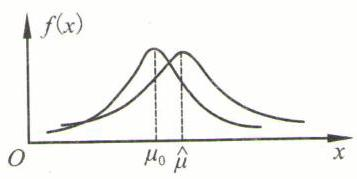
\includegraphics[width=0.3\textwidth]{bodyxb/src/bo_d20cdrf7aajc73bfmvhg_206_1130_560_357_179_0.jpg}
\end{center}


(第 106 题)

故至少需包装 4 袋葡萄糖,才能使 “至少有一袋包装好的葡萄糖重量正常” 的概

率大于 0.98 .

而 $E\left\lbrack  X\right\rbrack   = {np} = {0.6826n}$ ,故相应成本 $Y = X + 2\left( {n - X}\right)  =  - X + {2n}$ .

$E\left\lbrack  Y\right\rbrack   =  - E\left\lbrack  X\right\rbrack   + {2n} = {2n} - {0.6826n} = {1.3174n} \geq  {5.2696}$ ,所以相应成本的最小期望值为 5.2696 元.

(2)①如图所示,经计算得 $\widehat{\mu } = \bar{x} = {0.511}$ .

$\widehat{\mu } > {\mu }_{0} = {0.5}$ ,(绘图时只需保证 $\widehat{\mu }$ 在 ${\mu }_{0}$ 的右侧,且峰值略低于原图像峰值)

② $n = 9,{\mu }_{0} = {0.5},\widehat{\sigma } = {0.00972},\widehat{\mu } = \bar{x} = {0.511},\left| Z\right|  = \left| \dfrac{\widehat{\mu } - {\mu }_{0}}{\dfrac{\sigma }{\sqrt{n}}}\right|  = \dfrac{275}{81} \approx  {3.40} > {1.96}$

所以在犯错误概率不超过 0.05 的前提下, 认为该包装机工作异常, 应该进行调试.

107. B 提示: 正方形的面积与边长之间有着明确的等量关系, 不是相关关系, 故 B 正确.

108. D 提示: ${0.85} > {0.82} > {0.78} > {0.69}$ ,能体现出 $A,B$ 两变量有更强的线性相关性的是丁.

109. B 提示: 在一定年龄段内, 人体的脂肪含量与年龄之间有相关关系, A 错误.

汽车的重量和汽车每消耗 1 L 汽油所行驶的平均路程为负相关, B 正确.

吸烟量与健康水平为负相关, $C$ 错误.

气温与热饮销售状况为负相关, $D$ 错误.

110. A 提示:对于 A,散点图中的点从左向右是上升的,且在一条直线附近,是正相关.

对于 $B$ ,散点图中的点从左向右是下降的,且在一条直线附近,是负相关.

对于 $C,D$ ,没有明显的相关关系.

111. C 提示: 对于 $A,B$ ,由图可知北极年平均海冰面积既有增加又有减少,故 $A,B$ 错误.

\begin{center}
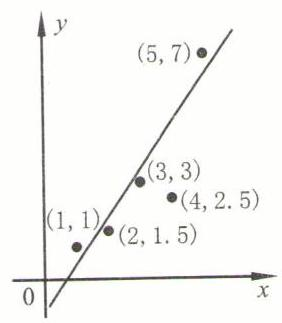
\includegraphics[width=0.2\textwidth]{bodyxb/src/bo_d20cdrf7aajc73bfmvhg_206_1222_1539_282_323_0.jpg}
\end{center}


(第 112 题)

对于 $C,D$ ,由图可知随着年平均二氧化碳浓度增加,北极年平均海冰面积总体呈下降趋势, 故 $C$ 正确, $D$ 错误.

112. C 提示: 在平面直角坐标系中画出五个点, $\left( {1,1}\right) ,\left( {2,1,5}\right) ,\left( {3,3}\right) ,\left( {4,2,5}\right) ,\left( {5,7}\right)$ ,如图,结果除去(4,2.5)之外,其余的点都在一条线附近,去掉这个点以后剩下的数据线性相关程度更高.

113. B 提示:

\begin{center}
\adjustbox{width=\textwidth}{
\begin{tabular}{|c|c|c|c|}
\hline
\phantom{X} & 喜欢 & 不喜欢 & 总计 \\
\cline{1-4}
男 & 30m & 20m & 50m \\
\cline{1-4}
女 & 20m & 30m & 50m \\
\cline{1-4}
总计 & 50m & 50m & 100m \\
\cline{1-4}
\hline
\end{tabular}
}
\end{center}

${\chi }^{2} = \dfrac{{100m}{\left( {900}{m}^{2} - {400}{m}^{2}\right) }^{2}}{{50} \times  {50} \times  {50} \times  {50}{m}^{4}} = {4m}.$

因为有 99.9\% 的把握认为性别与是否喜欢该学科有关,所以 ${4m} > {10},{828}$ ,解得 $m > {2.707}$ ,故 $m$ 的最小值为 3 . 从而 ${N}_{\min } = {300}$ .

114. A 提示:提出原假设 ${H}_{0}$ :该地青年人的低密度脂蛋白浓度与肥胖无关.

由题表知 ${\chi }^{2} = \dfrac{{100} \times  {\left( {10} \times  {15} - {10} \times  {65}\right) }^{2}}{{75} \times  {25} \times  {20} \times  {80}} \approx  {8.333} > {7.879},\therefore P\left( {{\chi }^{2} \geq  {k}_{0}}\right)  = {0.005}$ .

所以,在犯错误的概率不超过 0.5\%的前提下,认为 “该地青年人的低密度脂蛋白浓度与肥胖有关”.

115. 从图中可以看出, 总体来说, 热茶销量与气温之间具有明显的相关性, 气温越低热茶的销量往往越高.

\begin{center}
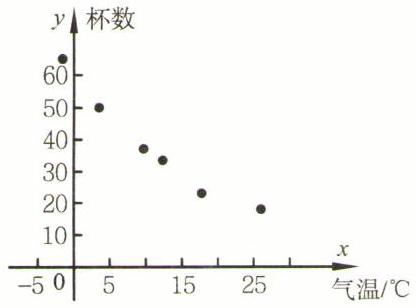
\includegraphics[width=0.3\textwidth]{bodyxb/src/bo_d20cdrf7aajc73bfmvhg_207_1006_319_416_308_0.jpg}
\end{center}


(第 115 题)

进一步地,通过计算器,可以求得 $r \approx   - {0.97}$ ,这说明热茶销量与气温之间具有很高的相关性.

116. 由题意得 $\bar{t} = 4,\mathop{\sum }\limits_{{i = 1}}^{7}{\left( {t}_{i} - \bar{t}\right) }^{2} = {28},\sqrt{\mathop{\sum }\limits_{{i = 1}}^{7}{\left( {y}_{i} - \bar{y}\right) }^{2}} = {0.55},\mathop{\sum }\limits_{{i = 1}}^{7}\left( {{t}_{i} - \bar{t}}\right) \left( {{y}_{i} - \bar{y}}\right)  =$  $\mathop{\sum }\limits_{{i = 1}}^{7}{t}_{i}{y}_{i} - \bar{t}\mathop{\sum }\limits_{{i = 1}}^{7}{y}_{i} = {40.17} - 4 \times  {9.32} = {2.89},r = \dfrac{2.89}{\sqrt{28} \times  {0.55}} \approx  {0.99}$ 说明 $y$ 与 $t$ 的线性相关程度相当高,可以用线性回归模型拟合 $y$ 与 $t$ 的关系. 117. (1) 样本中 10 个这种零件的横截面积的平均值 $\bar{x} = \dfrac{0.52}{10} = {0.052}$ , 样本中 10 个这种零件的耗材量的平均值 $\bar{y} = \dfrac{3.9}{10} = {0.39}$ . 由此可估算该学生制作的这种零件平均每个零件的横截面积为 ${0.052}{\mathrm{\;{mm}}}^{2}$ ,平均一个零件的耗材量为 ${0.39}{\mathrm{\;{mm}}}^{3}$ . (2)由表格中的参考数据和相关系数的公式, 可得 $r = \dfrac{\mathop{\sum }\limits_{{i = 1}}^{{10}}{x}_{i}{y}_{i} - {10}\bar{x}\bar{y}}{\sqrt{\left( {\mathop{\sum }\limits_{{i = 1}}^{{10}}{x}_{i}^{2} - {10}{\bar{x}}^{2}}\right) \left( {\mathop{\sum }\limits_{{i = 1}}^{{10}}{y}_{i}^{2} - {10}{\bar{y}}^{2}}\right) }} = \dfrac{{0.214} - {30} \times  {0.052} \times  {0.39}}{\sqrt{{1.491} - {36} \times  {10}^{-4}}} = \dfrac{1.15}{\sqrt{1.491}} \approx  {0.94},$ 所以这种零件的横截面积和耗材量的样本相关系数为 0.94 . 118. (1) 依题意, $r = \dfrac{\mathop{\sum }\limits_{{i = 1}}^{n}{x}_{i}{y}_{i} - n\bar{x}\bar{y}}{\sqrt{\left( {\mathop{\sum }\limits_{{i = 1}}^{n}{x}_{i}^{2} - n{\bar{x}}^{2}}\right) \left( {\mathop{\sum }\limits_{{i = 1}}^{n}{y}_{i}^{2} - n{\bar{y}}^{2}}\right) }} = \dfrac{{66.2} - 5 \times  3 \times  {4.8}}{\sqrt{{55} - 5 \times  {3}^{2}} \times  \sqrt{{118.7} - 5 \times  {4.8}^{2}}} \approx   - {0.9804}$ ,所以线性相关程度较高. (2) $\widehat{a} = \dfrac{\mathop{\sum }\limits_{{i = 1}}^{n}{x}_{i}{y}_{i} - n\overline{xy}}{\mathop{\sum }\limits_{{i = 1}}^{n}{x}_{i}^{2} - n{\bar{x}}^{2}} =  - {0.58},\widehat{b} = \bar{y} - \widehat{a}\bar{x} = {6.54}$ ,所以 $y =  - {0.58x} + {6.54}$ . 当 $x = 6$ 时, $y =  - {0.58} \times  6 + {6.54} = {3.06}$ 万吨

119. (1) 由题意,效果不明显的青年有 ${61} + {75} + 7 + 7 = {150}$ ,

效果明显的青年有 ${40} + {50} + {100} + {60} = {250}$ ,

效果不明显的中年有 ${55} + {43} + 5 + 7 = {110}$ ,

效果明显的中年有 ${50} + {90} + {100} + {50} = {290}$ ,

故 $2 \times  2$ 列联表如下:

\begin{center}
\adjustbox{width=\textwidth}{
\begin{tabular}{|c|c|c|c|}
\hline
\multirow{2}{*}{效果} & \multicolumn{2}{|c|}{年龄} & \multirow{2}{*}{合计} \\
\cline{2-3}
 & 青年 & 中年 &  \\
\cline{1-4}
效果不明显 & 150 & 110 & 260 \\
\cline{1-4}
效果明显 & 250 & 290 & 540 \\
\cline{1-4}
合计 & 400 & 400 & 800 \\
\cline{1-4}
\hline
\end{tabular}
}
\end{center}

(2)原假设 ${H}_{0}$ :治疗效果与年龄无关,确定显著性水平 $\alpha  = {0.01}$ .

${\chi }^{2} = \dfrac{{800} \times  {\left( {150} \times  {290} - {110} \times  {250}\right) }^{2}}{{260} \times  {540} \times  {400} \times  {400}} \approx  {9.117} > {6.635},$

否定 ${H}_{0}$ ,即认为治疗效果与年龄有关.

120. B 提示: 左侧两图是正相关,样本相关系数大于 0 ,则 ${r}_{1} > 0,{r}_{3} > 0$ .

右侧两图是负相关,样本相关系数小于 0,则 ${r}_{2} < 0,{r}_{4} < 0$ .

下方两图的点相对更加集中,所以相关性较强,上方两图的点相对分散一些,所以相关性较弱,由此可得 ${r}_{4} < {r}_{2} < 0 < {r}_{1} < {r}_{3}$ .

121. $C$ 提示: 由变量 $X$ 与 $Y$ 相对应的一组数据为 $\left( {{10},1}\right) ,\left( {{11.3},2}\right) ,\left( {{11.8},3}\right) ,\left( {{12.5},4}\right) ,\left( {{13},5}\right)$ ,可得变量 $X$ 与 $Y$ 之间正相关,所以 ${r}_{1} > 0$ .

由变量 $U$ 与 $V$ 相对应的一组数据为 (10.5). (11.3.4). (11.8.3). (12.5.2). (13.1),可知变量 $U$ 与 $V$ 之间负相关,所以 120 D. 提示. 对于选项 A,去掉图中右下方的点 $A$ 后,两个变量还是负相关, A 错误. 对于选项 ${BCD}$ ,去掉图中右下方的点 $A$ 后,相对来说数据会集中,相关程度会更高, 但因为是负相关,相关系数会更接近一1,线性相关系数会变小,故D正确, DC相应 123.C 提示: 设男、女大学生各有 $m$ 人,根据题意画出 $2 \times  2$ 列联表如下:

\begin{center}
\adjustbox{width=\textwidth}{
\begin{tabular}{|c|}
\hline
不看营养说明 급 yi 看营养说明 $\dfrac{1}{5}m$  $m$ 男 $\dfrac{4}{5}m$  $\dfrac{2}{5}m$  $m$ 女 $\dfrac{3}{5}m$  ${2m}$  $\dfrac{3}{5}m$ 合计 $\dfrac{7}{5}m$ \\
\cline{1-1}
\hline
\end{tabular}
}
\end{center}

所以 ${\chi }^{2} = \dfrac{{2m}{\left( \dfrac{4}{5}m \times  \dfrac{2}{5}m - \dfrac{3}{5}m \times  \dfrac{1}{5}m\right) }^{2}}{\dfrac{7}{5}m \times  \dfrac{3}{5}m \times  m \times  m} = \dfrac{2m}{21}$ ,因为有 99.9\%的把握认为性别与是否看营养说明有关,

所以 $\dfrac{2m}{n} > {10.828}$ ,解得 ${2m} > {227.388}$ ,所以总人数至少为 228.

124.D. 提示: 由于 $\bar{x} = 3,\bar{z} = {3.98}$ ,则 ${3.98} =  - {0.062} \times  3 + t$ . 解得 $t = {4.166}$ ,则 ${C}_{20}^{1}{C}_{20}^{1} + {C}_{20}^{2}$ \_\_\_\_\_59

125. (1)记“任选两名患者,至少一名患者在实验组”为事件 $A$ ,则 $P\left( A\right)  = \dfrac{2}{{C}_{40}^{2}} = {78}$ .

记“一名患者在对照组”为事件 $B$ ,则 $P\left( {A \cap  B}\right)  = \dfrac{{C}_{20}^{1}{C}_{20}^{1}}{{C}_{40}^{2}} = \dfrac{20}{39}$ ,所以 $P\left( {B \mid  A}\right)  = \dfrac{P\left( {A \cap  B}\right) }{P\left( A\right) } = \dfrac{\bar{39}}{58} = \dfrac{40}{59}$ .

(2)①传题意,这 40 个数据的中位数是将两组数据合在一起,从小到大排序后第 20 位与第 21 位数据的平均数.

可得第 20 位数据为:23.4,第 21 位数据为:23.6,所以 $m = \dfrac{{23.4} + {23.0}}{2} = {23.5}$ .

\begin{center}
\adjustbox{width=\textwidth}{
\begin{tabular}{|c|c|c|}
\hline
列联表为: 药物 $A$ 对照组 实验组 合计 & 疾病 $B$ 指标数据 $\geq  m$ 指标数据 $< m$ 14 6 6 14 20 20 & 合计 20 20 40 \\
\cline{1-3}
\hline
\end{tabular}
}
\end{center}

②原假设 ${H}_{0}$ : 药物 $A$ 对治疗疾病 $B$ 无效,确定显著性水平 $\alpha  = {0.01}$ ,计算 ${\chi }^{2} = \dfrac{{40}{\left( 6 \times  6 - {14} \times  {14}\right) }^{2}}{{20} \times  {20} \times  {20} \times  {20}} = {6.4} < {6.635}$ .

没有充分证据推断 ${H}_{0}$ 不成立,因此可认为药物 $A$ 对治疗疾病 $B$ 无效.

126. (1) 由表中数据可得 $\overline{x} = \dfrac{1 + 2 + 3 + 4 + 5}{5} = 3,\overline{y} = \dfrac{{77} + {84} + {93} + {96} + {100}}{5} = {90}$ ,

则 $\widehat{a} = \dfrac{\mathop{\sum }\limits_{{i = 1}}^{5}\left( {{x}_{i} - \bar{x}}\right) \left( {{y}_{i} - \bar{y}}\right) }{\mathop{\sum }\limits_{{i = 1}}^{5}{\left( {x}_{i} - \bar{x}\right) }^{2}} = {5.8},\widehat{b} = \bar{y} - \widehat{a}\bar{x} = {90} - {5.8} \times  3 = {72.6}$ ,

所以 $y$ 关于 $x$ 的一元线性回归方程是 $y = {5.8x} + {72.6}$ ,

令 $x = 7$ ,得 $\widehat{y} = {113.2}$ ,所以估计当年 2 月 21 日在该店购物的人数为 115 人. (2) $2 \times  2$ 列联表如下:

\begin{center}
\adjustbox{width=\textwidth}{
\begin{tabular}{|c|c|c|c|}
\hline
$2 \times  2$ 列联表如下: 年龄 参与过网上购物 未参与过网上购物 合计 & 不低于 40 岁 30 20 50 & 低于 40 岁 120 30 150 & 合计 150 50 200 \\
\cline{1-4}
\hline
\end{tabular}
}
\end{center}

提出原假设 ${H}_{0}$ : 参加网上购物和年龄无关,

确定显著性水平 $\alpha  = {0.005}$ ,计算 ${\chi }^{2} = \dfrac{{200} \times  {\left( {30} \times  {30} - {120} \times  {20}\right) }^{2}}{{150} \times  {50} \times  {50} \times  {150}} = 8 > {7.879}$ ,否定原假设,即可以认为参加网上购

物和年龄有关.

127. (1) 因为 $r = \dfrac{\mathop{\sum }\limits_{{i = 1}}^{{10}}\left( {{x}_{i} - \bar{x}}\right) \left( {{y}_{i} - \bar{y}}\right) }{\sqrt{\mathop{\sum }\limits_{{i = 1}}^{{10}}{\left( {x}_{i} - \bar{x}\right) }^{2}\mathop{\sum }\limits_{{i = 1}}^{{10}}{\left( {y}_{i} - \bar{y}\right) }^{2}}} = \dfrac{\mathop{\sum }\limits_{{i = 1}}^{{10}}{x}_{i}{y}_{i} - {10}\bar{x}\bar{y}}{\sqrt{\left( {\mathop{\sum }\limits_{{i = 1}}^{{10}}{x}_{i}^{2} - {10}{\bar{x}}^{2}}\right)  \times  \left( {\mathop{\sum }\limits_{{i = 1}}^{{10}}{y}_{i}^{2} - {10}{\bar{y}}^{2}}\right) }}$ ,

代入已知数据,得 $r \approx  {0.98}$ . 所以汛期遥测雨量 $y$ 与人工测雨量 $x$ 有线性相关关系

(2)依题意,“ I 类误差”有 5 组,“ II 类误差”有 3 组,“ III 类误差”有 2 组.

若从 “ I 类误差” 和 “ II 类误差” 数据中抽取 3 组,抽到 “ I 类误差” 的组数 $X$ 的所有可能取值为 0.1,2.3

则 $P\left( {X = 0}\right)  = \dfrac{{C}_{3}^{3}}{{C}_{8}^{3}} = \dfrac{1}{56},P\left( {X = 1}\right)  = \dfrac{{C}_{5}^{1}{C}_{3}^{2}}{{C}_{8}^{3}} = \dfrac{15}{56}$ ,

$P\left( {X = 2}\right)  = \dfrac{{C}_{5}^{2}{C}_{3}^{1}}{{C}_{8}^{3}} = \dfrac{30}{56} = \dfrac{15}{28},P\left( {X = 3}\right)  = \dfrac{{C}_{5}^{3}{C}_{3}^{0}}{{C}_{8}^{3}} = \dfrac{5}{28}.$

所以 $X$ 的概率分布为 $\left( \begin{matrix} 0 & 1 & 2 & 3 \\  \dfrac{1}{56} & \dfrac{15}{56} & \dfrac{15}{28} & \dfrac{5}{28} \end{matrix}\right)$ .

从而 $E\left\lbrack  X\right\rbrack   = \dfrac{15}{8}$ .

128. (1) $2 \times  2$ 列联表如下:

\begin{center}
\adjustbox{width=\textwidth}{
\begin{tabular}{|c|c|c|c|}
\hline
\phantom{X} & 汽车日流量 $< {1500}$ & 汽车日流量 $x \geq  {1500}$ & 合计 \\
\cline{1-4}
PM2.5 的平均浓度 $y < {100}$ & 16 & 8 & 24 \\
\cline{1-4}
PM2.5 的平均浓度 $y \geq  {100}$ & 6 & 20 & 26 \\
\cline{1-4}
合计 & 22 & 28 & 50 \\
\cline{1-4}
\hline
\end{tabular}
}
\end{center}

提出原假设 ${H}_{0} :$ " $\mathrm{{PM}}{2.5}$ 平均浓度不小于 ${100\mu }\mathrm{g}/{\mathrm{m}}^{3}$ " 与 “汽车日流量不少于 1500 辆”无关.

因为 ${\chi }^{2} = \dfrac{{50} \times  {\left( {16} \times  {20} - 8 \times  6\right) }^{2}}{{24} \times  {26} \times  {22} \times  {28}} \approx  {9.62} \in  \left( {{7.879},{10.828}}\right)$ ,所以至少有 99.5 \%的把握 (但还不能有 99.9 \% 的把握) 认为 “PM2.5 平均浓度不小于 100 $\mu \mathrm{g}/{\mathrm{m}}^{3}$ ” 与 “汽车日流量不小于 1500 辆” 有关.

(2)因为回归方程为 $y = {0.12x} - {73.36}$ ,所以 $\widehat{a} = \dfrac{\mathop{\sum }\limits_{{i = 1}}^{{50}}\left( {{x}_{i} - \bar{x}}\right) \left( {{y}_{i} - \bar{y}}\right) }{\mathop{\sum }\limits_{{i = 1}}^{{50}}{\left( {x}_{i} - \bar{x}\right) }^{2}} = {0.12}$ .

又因为 $\sqrt{\dfrac{\mathop{\sum }\limits_{{i = 1}}^{{50}}{\left( {x}_{i} - \bar{x}\right) }^{2}}{50}} = {252},\sqrt{\dfrac{\mathop{\sum }\limits_{{i = 1}}^{{50}}{\left( {y}_{i} - \bar{y}\right) }^{2}}{50}} = {36}$ ,

所以 $r = \dfrac{\mathop{\sum }\limits_{{i = 1}}^{{50}}\left( {{x}_{i} - \bar{x}}\right) \left( {{y}_{i} - \bar{y}}\right) }{\sqrt{\mathop{\sum }\limits_{{i = 1}}^{{50}}{\left( {x}_{i} - \bar{x}\right) }^{2}\mathop{\sum }\limits_{{i = 1}}^{{50}}{\left( {y}_{i} - \bar{y}\right) }^{2}}} = \widehat{a} \cdot  \sqrt{\dfrac{\mathop{\sum }\limits_{{i = 1}}^{{50}}{\left( {x}_{i} - \bar{x}\right) }^{2}}{\mathop{\sum }\limits_{{i = 1}}^{{50}}{\left( {y}_{i} - \bar{y}\right) }^{2}}} = {0.12} \times  \dfrac{252}{36} = {0.84}$ .

129. 由 $y = a{\mathrm{e}}^{-\dfrac{b}{x}}$ 得 $\ln y =  - \dfrac{b}{x} + \ln a$ ,设 $t = \dfrac{1}{x},s = \ln y$ ,则 $s =  - {bt} + \ln a$ ,

由已知数据得:

\begin{center}
\adjustbox{width=\textwidth}{
\begin{tabular}{|c|c|c|c|c|c|c|c|c|c|c|}
\hline
编号 & 1 & 2 & 3 & 4 & 5 & 6 & 7 & 8 & 9 & 10 \\
\cline{1-11}
$t$ & 20 & 16.667 & 14. 286 & 10 ` & 7. 143 & 5 & 4 & 3.226 & 2.632 & 2.326 \\
\cline{1-11}
$S$ & -2.303 & -1.966 & -1.470 & -0.994 & -0.528 & -0.236 & 0 & 0.113 & 0.174 & 0.223 \\
\cline{1-11}
\hline
\end{tabular}
}
\end{center}

$\bar{t} = \dfrac{{20} + {16.667} + \cdots  + {2.326}}{10} = {8.528},$

$\bar{s} = \dfrac{\left( {-{2.303}}\right)  + \left( {-{1.966}}\right)  + \cdots  + {0.223}}{10} =  - {0.6987},$

回归方程为 $s =  - {0.1456t} + {0.543}$ .

所以 $a$ 的估计值为 ${\mathrm{e}}^{0.543} \approx  {1.7212},b$ 的估计值为 0.1456 .